\documentclass[12pt]{article}
\usepackage{lingmacros}
\usepackage{tree-dvips}
\usepackage[a4paper, total={6in, 9in}]{geometry}
\usepackage[parfill]{parskip}
\usepackage{amsmath}
\usepackage{hyperref}
\usepackage{cleveref}
\usepackage{autonum}
\usepackage{amsmath}
\usepackage{pythonhighlight}
\usepackage{graphicx}
\usepackage{caption}
\usepackage{subcaption}
\usepackage[export]{adjustbox}
\graphicspath{ {/home/user/Desktop/LaTeX} }
\begin{document}
\begin{figure}[!tbp]

\section*{\centering{MATH3001: Everything We've Learnt So Far...}}
\medskip 
\subsection*{Chapter 1}
Chapter 1 provides an introduction to Monte Carlo methods, specifically, how we can use randomness to produce accurate results. Random numbers can be used for statistical sampling (also called “Monte Carlo sampling”). A common application of this is in numerical integration. For integration in one dimension, other numerical integration methods (such as Simpson’s and Trapezium rule) are usually more efficient than Monte Carlo Methods. But for multidimensional integrals, Monte Carlo methods become competitive, and for very large numbers of dimensions these are the only practical method for numerical integration.

\subsection*{Homework Task 1}
In Homework Task 1, we used the python code provided in the session to evaluate the mean and variance of a random sample drawn from probability distributions.
\medskip 
\medskip 

  \begin{subfigure}[b]{0.4\textwidth}
    \includegraphics[width=\textwidth]{Normal_1000.png}
    \caption{$N$ = $1,000$}
    \label{fig:f1}
  \end{subfigure}
  \hfill
  \begin{subfigure}[b]{0.41\textwidth}
    \includegraphics[width=\textwidth]{Normal_10000.png}
    \caption{$N$ = $10,000$}
    \label{fig:f2}
  \end{subfigure}
  \caption{Random Sampling from a Normal Distribution}
\end{figure}

In Figure 1, we see that as you increase the value of $N$, the closer to the Normal Distribution the random sampling is. Like the Law of Large Numbers, this is a phenomenon we expect. 

We can analyse how good these random sampling approximations of the mean and variance are. First, we will plot the approximations of the mean for different values of N for both the exponential and normal distributions, as can be seen in Figure 2. 

We observe that, even for $N = 100,000$, the Normal Distribution and Exponential Distribution do not calculate the exact value for the mean. In particular, we see that the Exponential Distribution is actually better at estimating the true value of the mean when compared to the Normal Distribution. 

Although these distributions do not give an output that is the exact mean, we can incorporate percentage values and consider for what values of N we need to be within a particular percentage of the mean. 

\begin{figure}[h!]
  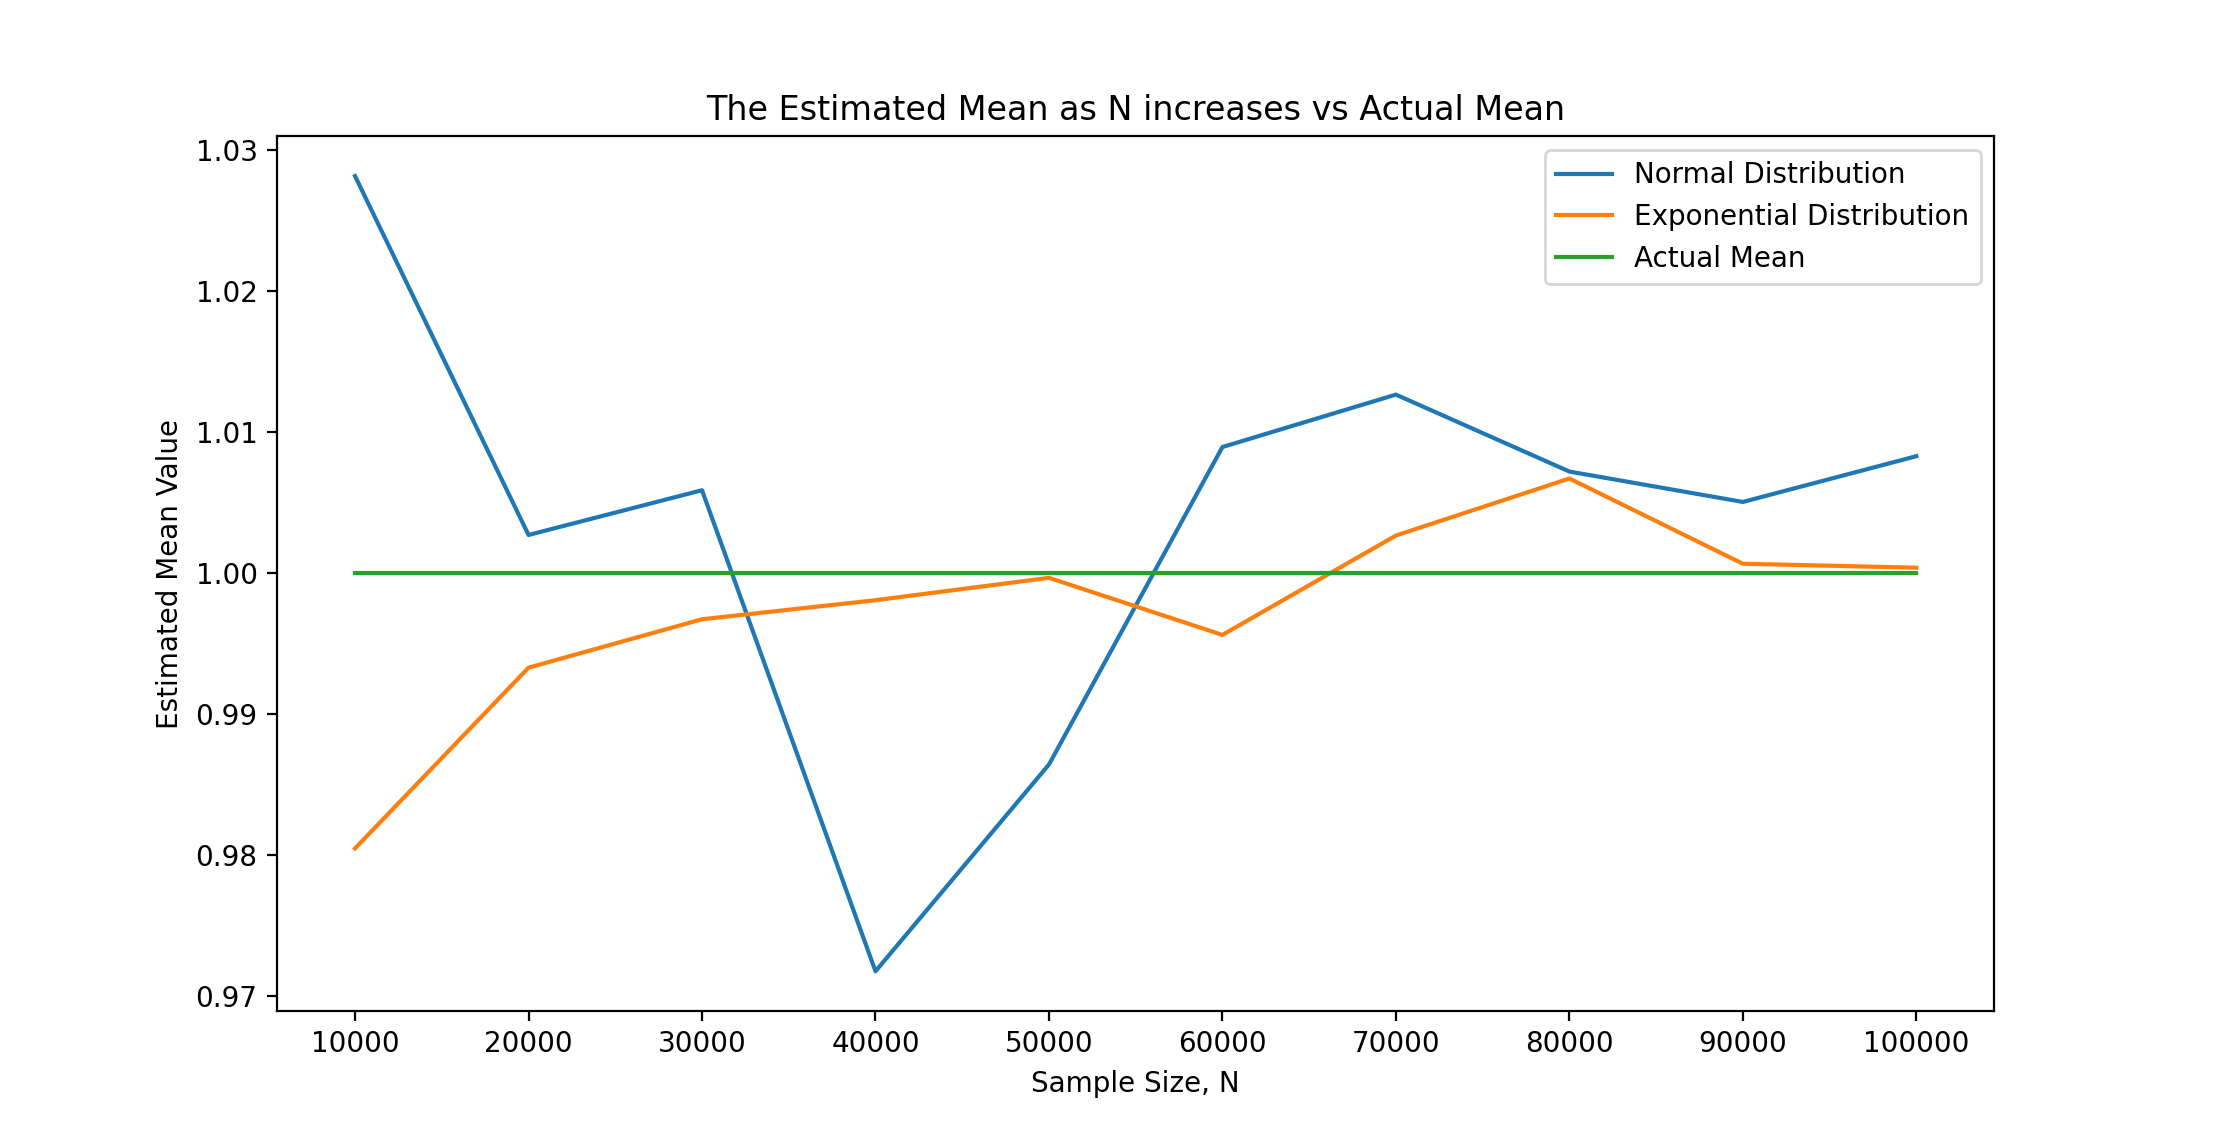
\includegraphics[scale=0.45, center]{Estimated Mean, 10,000 to 100,000}
  \caption{Estimated Mean as N Increases vs Actual Mean}
  \label{fig:estimated_mean}
\end{figure}

In Figure 3, we observe the effect of estimating the mean within a percentage value, as can be seen by the red lines. In this example, we used a 5 percent error estimation for the Normal Distribution and Exponential Distribution.

\begin{figure}[h]
\begin{subfigure}{0.5\textwidth}
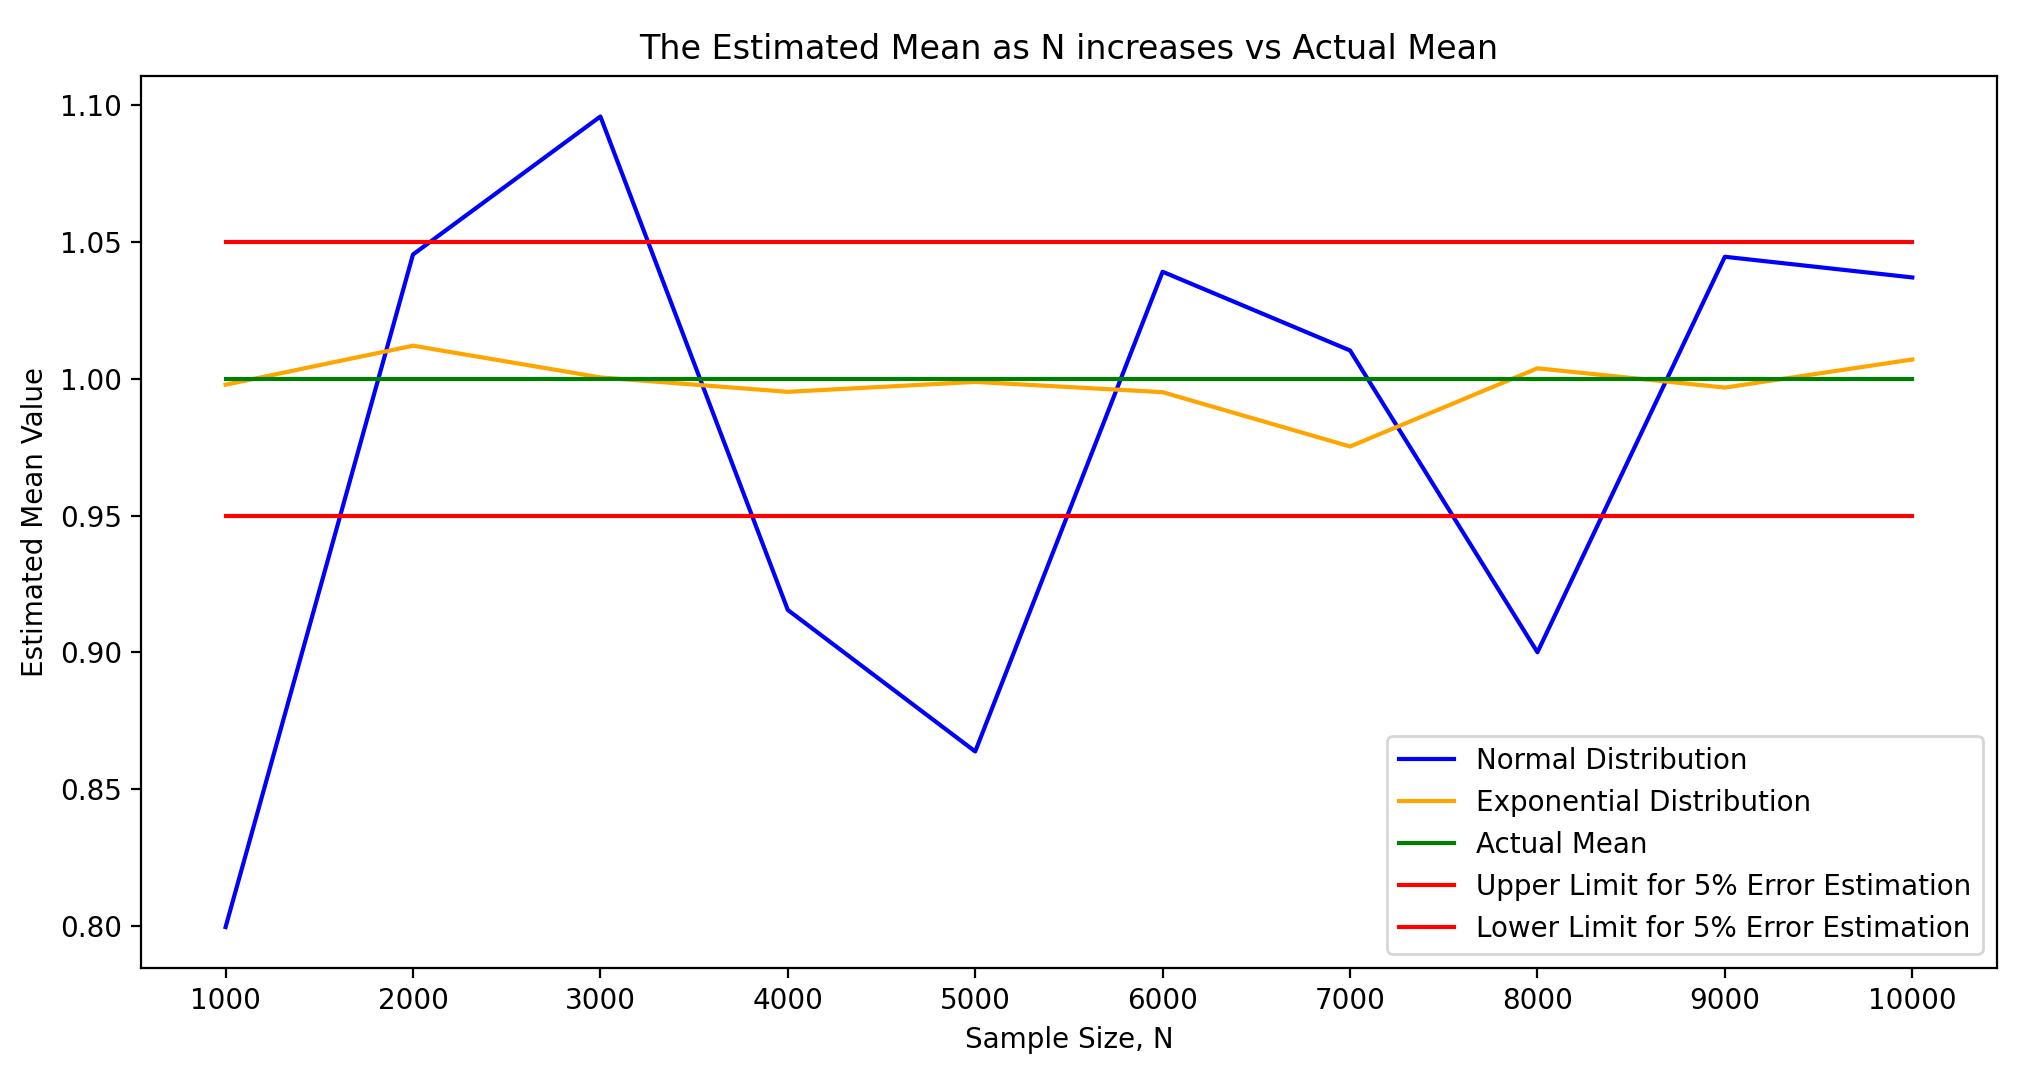
\includegraphics[width=1\linewidth, left]{1,000 to 10,000 5 percent error.png} 
\caption{$N = 10,000$}
\label{fig:subim1}
\end{subfigure}
\begin{subfigure}{0.5\textwidth}
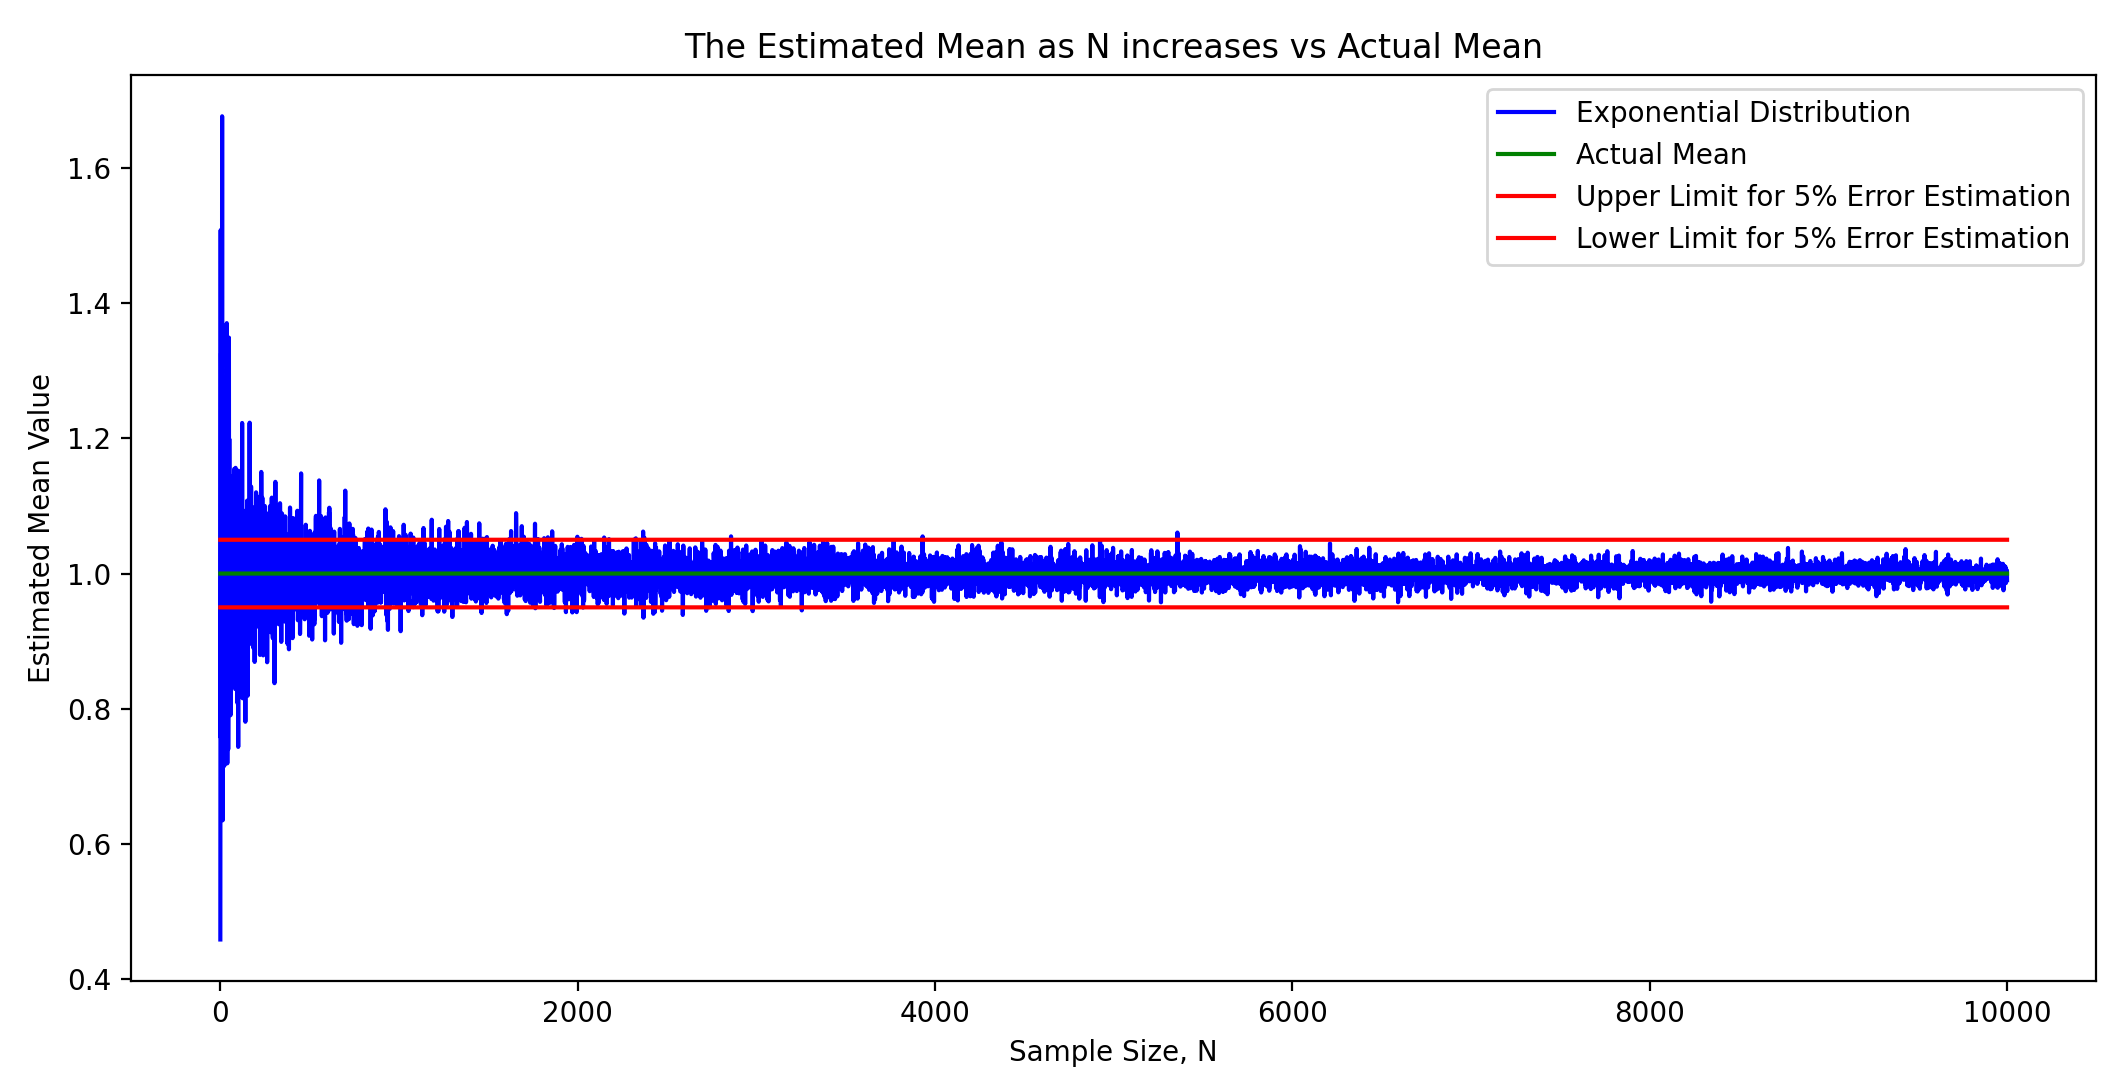
\includegraphics[width=1.03\linewidth]{Exponential N = 10,000.png}
\caption{$N = 1,000,000$}
\label{fig:subim2}
\end{subfigure}
\caption{Estimated Mean Within a Percentage Range}
\label{fig:image2}
\end{figure}

It is clear that as N is increased, the estimated mean lies within the upper and lower limit of the percentage error estimation. Although this is intuitive, it allows us to consider the standard error of the mean and then observe what minimum N value we need to be within a particular error percentage. 

We now consider the standard error of the mean, which can be defined as:
\begin{align}
\sigma\textsubscript{$\langle x\rangle$\textsubscript{$N$}}  = \frac{\sigma\textsubscript{$x$}}{\sqrt{N}}
\end{align}
where $N$ is the number of samples, $\sigma\textsubscript{$x$}$ is the actual mean and $\langle x\rangle\textsubscript{$N$}$ is the estimated mean for $N$ samples.

We can now plot the standard error of the mean for different distributions and increasing values of N. As can be seen in Figure 4. 
 
\begin{figure}[h!]
  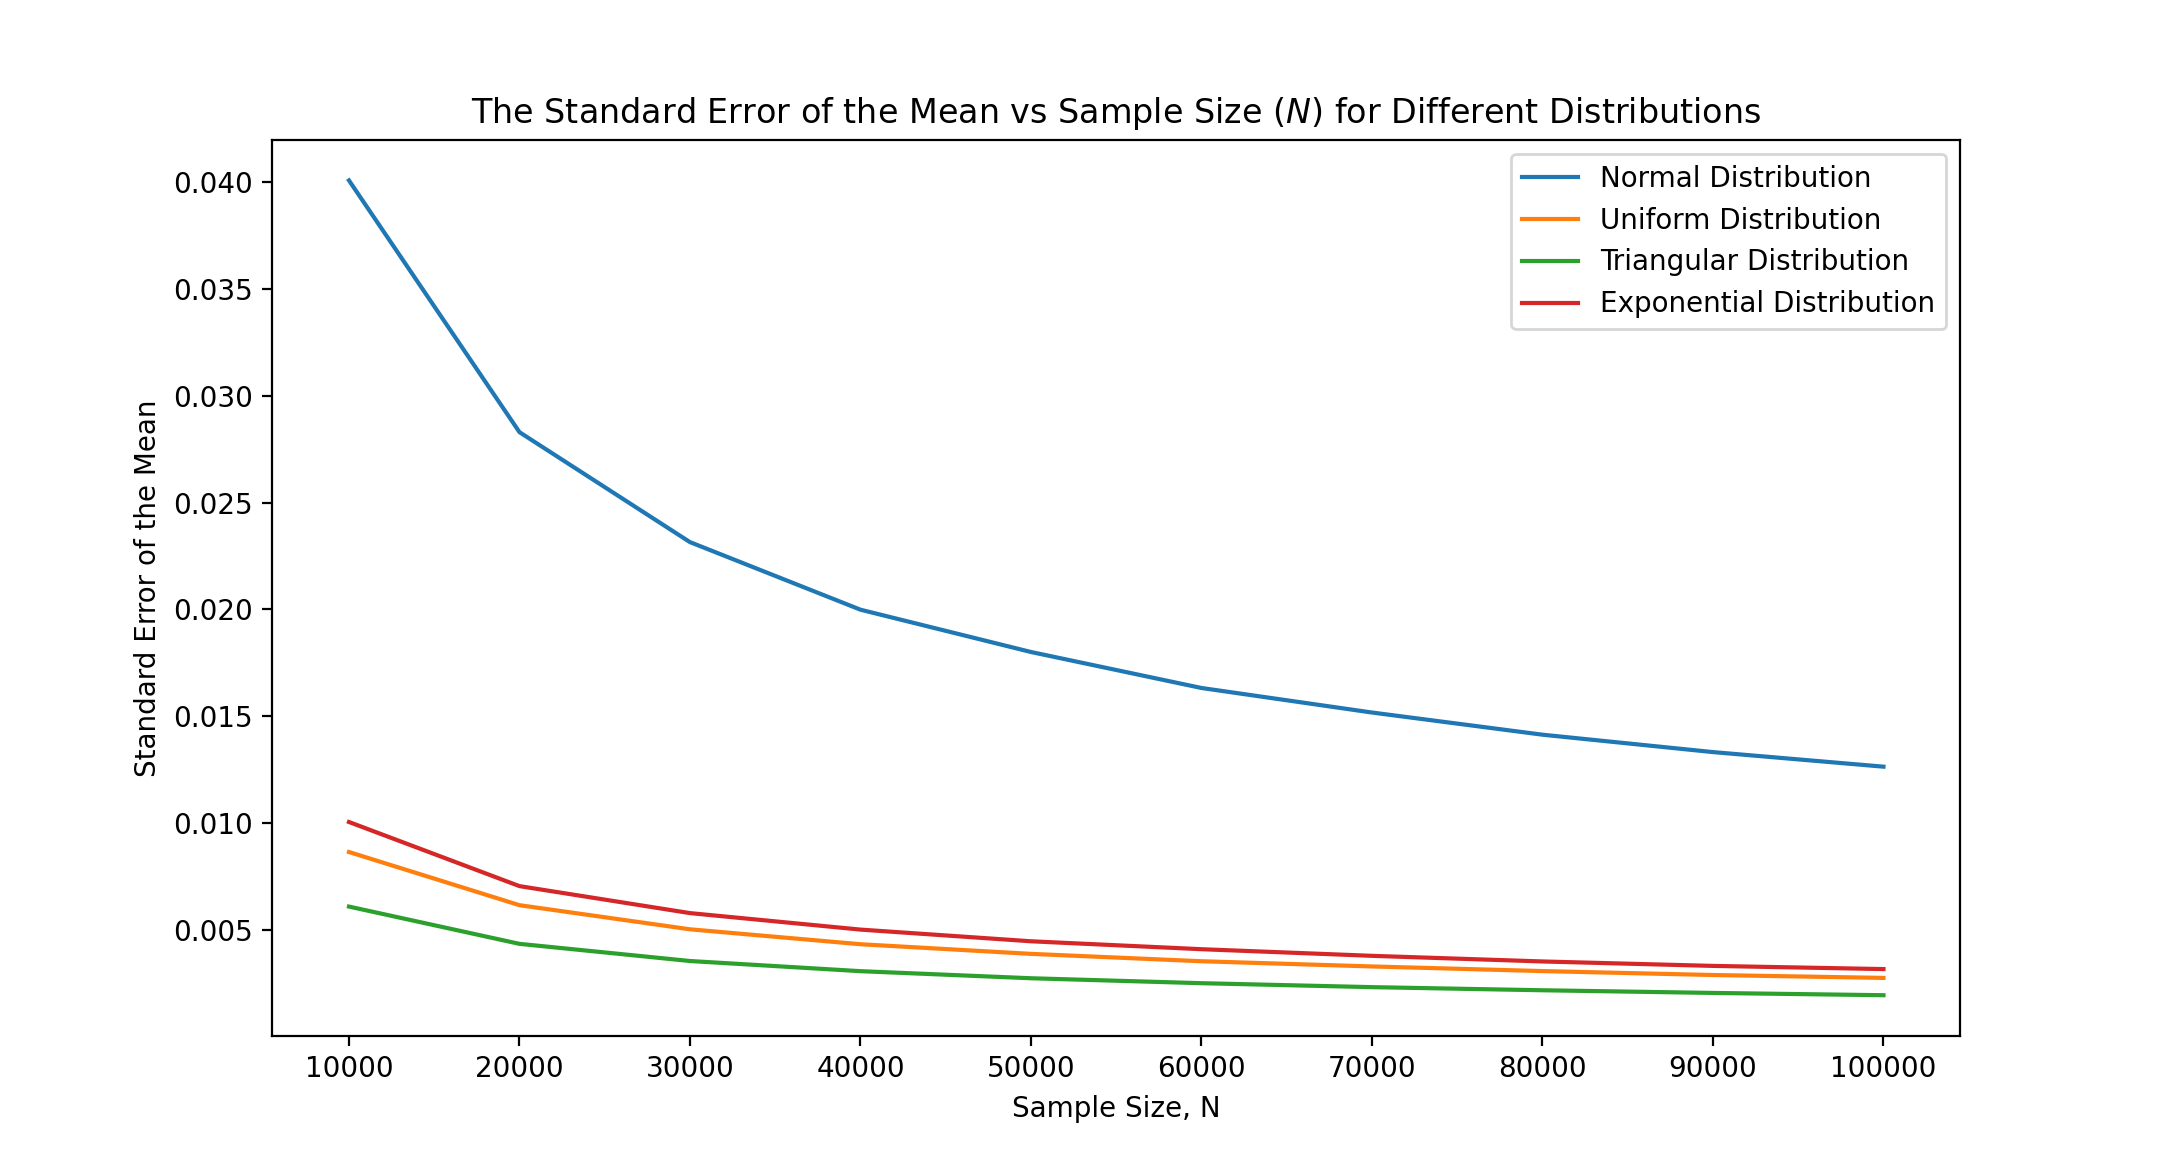
\includegraphics[scale=0.45, center]{10,000 to 100,000.png}
  \caption{Standard Error of the Mean for Different Distributions}
  \label{fig:estimated_mean}
\end{figure}

These distributions each have different parameters which gives rise to the different convergence rates. Again, we notice that as we increase N, the standard error of the mean decreases. 

We can use the standard error of the mean formula to calculate the minimum value of $N$ needed for the estimate to lie within a percentage of the true mean.

\subsubsection*{An Example}
Let's say we have \[
  X \sim \mathcal{N}(0,1)\,.
\]
What is the minimum value of $N$ needed for our estimated mean to be within a 0.5 percent standard error of the actual mean?

Rearranging the formula for the standard error of the mean, we have 
 

\begin{align}
N  &= (\frac{\sigma\textsubscript{$x$}}{\sigma\textsubscript{$\langle x\rangle$\textsubscript{$N$}}})^2\\\\
&= (\frac{1}{0.005})^2 \\\\
&= 40,000
\end{align}

Thus, the minimum value of $N$ needed to ensure our estimated mean would be within a 0.5 percent standard error of the mean is $N = 40,000$!

\subsection*{Chapter 2}
\subsection*{Monte Carlo Integration}

In Chapter 2, we extend Monte Carlo methods to look at integration. We then compare these methods with other quadrature methods like the Simpson's Rule and the Trapezium Rule. 

In Monte Carlo integration, the points are chosen randomly from a distribution. Since the mean value of f can be defined as
\begin{equation}
\langle f\rangle = \frac{1}{b-a}\int_{a}^{b} f(x) \,dx 
\end{equation}

we can determine the value of the integral by sampling f to find its mean value. Thus if we draw $N$ points,  $x\textsubscript{$1$}$,... $x\textsubscript{$N$}$ from a uniform distribution in the interval [a, b] then we can estimate the integral as,
\begin{equation}
\int_{a}^{b} f(x) \,dx \approx \frac{(b-a)}{N}\sum_{i=1}^{N} f(x_{i})\,
\end{equation}

Furthermore we can also estimate the error, by taking the square root of the mean
squared error as
 \begin{align} 
\frac{(b-a)}{\sqrt{N}}\sigma
\end{align}

where $\sigma^2$ is the variance of $f$ over the interval. This means that the accuracy of the estimate improves as the square root of the number of points sampled.

\subsection*{Multi-dimensional Integration}

As will be seen in the following answers to the Homework Tasks, there are better ways of integrating in one-dimension than Monte-Carlo (MC) methods.

In the notes, there is a comment on quadrature schemes for multi-dimensional examples. The consensus is that for the Simpson's Rule and Trapezium Rule, the total error will scale as $N^\frac{-1}{D}$. So when $D$ is large, the convergence is very slow. Even where we have a rectangular domain over which the function is differentiable the convergence rate we decrease as the number of dimensions increases. This is the “curse of dimensionality”.

For Monte Carlo Sampling:

The integral can be estimated as,
 \begin{align} 
\int\limits_V f(\mathbf{x}) \, dx \approx \frac{V}{N}\sum_{i=1}^{N} f(\mathbf{x}_{i})\, \pm V\frac{\sigma}{\sqrt{N}}
\end{align}

Hence, the error scales as $N^{\frac{-1}{2}}$ irrespective of the number of dimensions. 

\subsection*{Homework Task 2 (i)}

For a general function $f(x)$ obtain a formula for $\sigma$ and hence an error estimate.

\subsubsection*{Answer}

From the provided notes, we define the mean of a function $f(x)$,  $\langle f\rangle$ as:
\begin{equation}
\langle f\rangle = \frac{1}{b-a}\int_{a}^{b} f(x) \,dx 
\end{equation}
By intuition, we can deduce:
\begin{equation}
\langle f^2\rangle = \frac{1}{b-a}\int_{a}^{b} f(x)^2 \,dx 
\end{equation}

It is clear to see that the formula for $\sigma$ is:
\begin{equation}
\sigma =  \sqrt{{\langle f^2\rangle} - {\langle f\rangle ^2}}
\end{equation}

Using these results, it is easy to see that an unbiased estimate for the standard deviation of the random integration, $\sigma\textsubscript{$\langle f\rangle$\textsubscript{$N$}}$, (which is also denoted as the standard error component while using Monte Carlo integration), is the following:

\begin{equation}
\sigma\textsubscript{$\langle f\rangle$\textsubscript{$N$}} = \sqrt{\frac{
\langle f^2\rangle - \langle f\rangle ^2 }{N}}
\end{equation}

This is the formula for the error estimate. 

\subsection*{Homework Task 2 (ii)}

How does this compare with quadrature schemes such as the trapezium rule or Simpson’s rule? Write a program to estimate $\frac{1}{2}\int_{0}^{2} cos^2(x) \,dx$ using Monte-Carlo sampling. Compare the answer with the trapezium and/or Simpson’s rule. Is Monte-Carlo sampling a good way to estimate this integral?

\subsubsection*{Answer}

For most of the 1D integration, the quadrature schemes such as Simpson's Rule and Trapezium Rule perform better than the Monte Carlo method. For integration, the Monte Carlo method is usually used for high dimensional cases, like 3D integration or even higher than 3D. \par

Now, we use Monte Carlo Integration to solve the following integral,
\begin{align}
I = \frac{1}{2}\int_{0}^{2} cos^2(x) \,dx
\end{align}

We have produced code in Python that allows us to accurately estimate this integral using Monte Carlo methods. Below is a visual representation of $N$ = 1000 individual estimates. It is worth including this graph as it represents the randomness of these estimates. 
 
\begin{figure}[h!]
  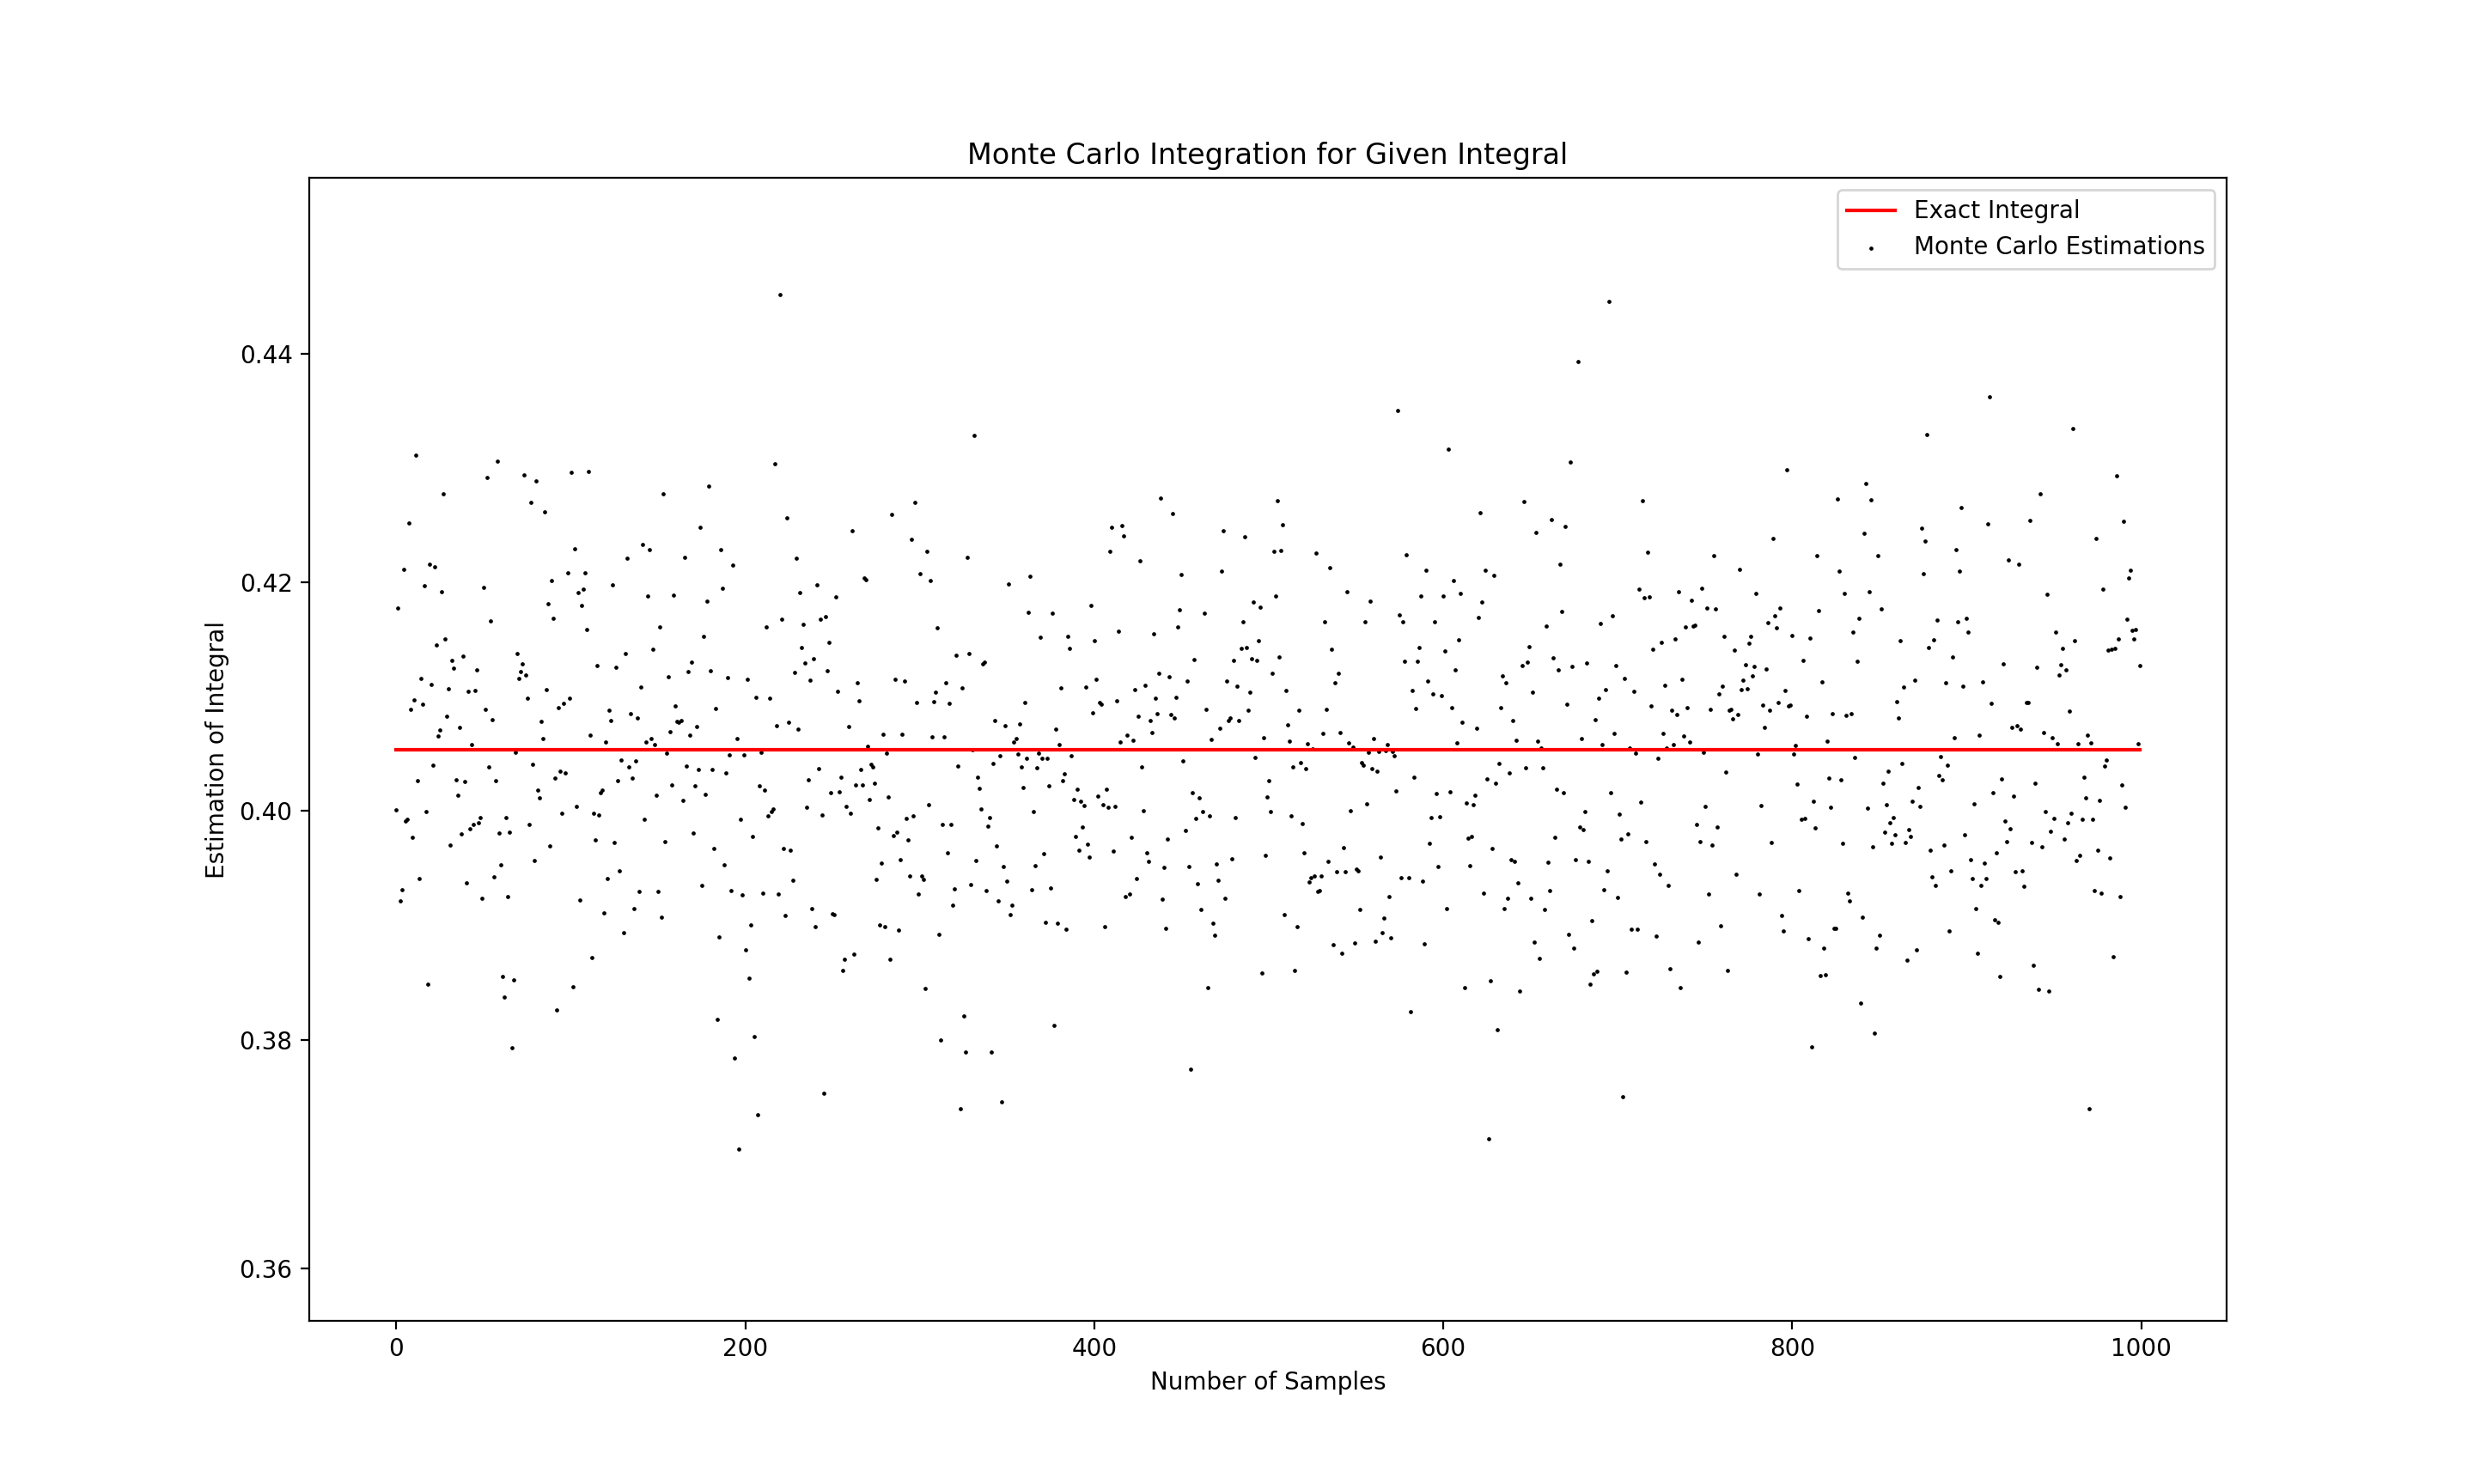
\includegraphics[scale=0.35, center]{HW1}
  \caption{Monte Carlo Integration for the Given Integral}
  \label{fig:mc_randomness}
\end{figure}


We notice that each estimation is within a small region above, below or exactly on the exact integral. To take this further, we could calculate the average of all $N = 1000$ estimates and plot the error versus $N$. This can be seen in Figure 6.

\begin{figure}[h!]
  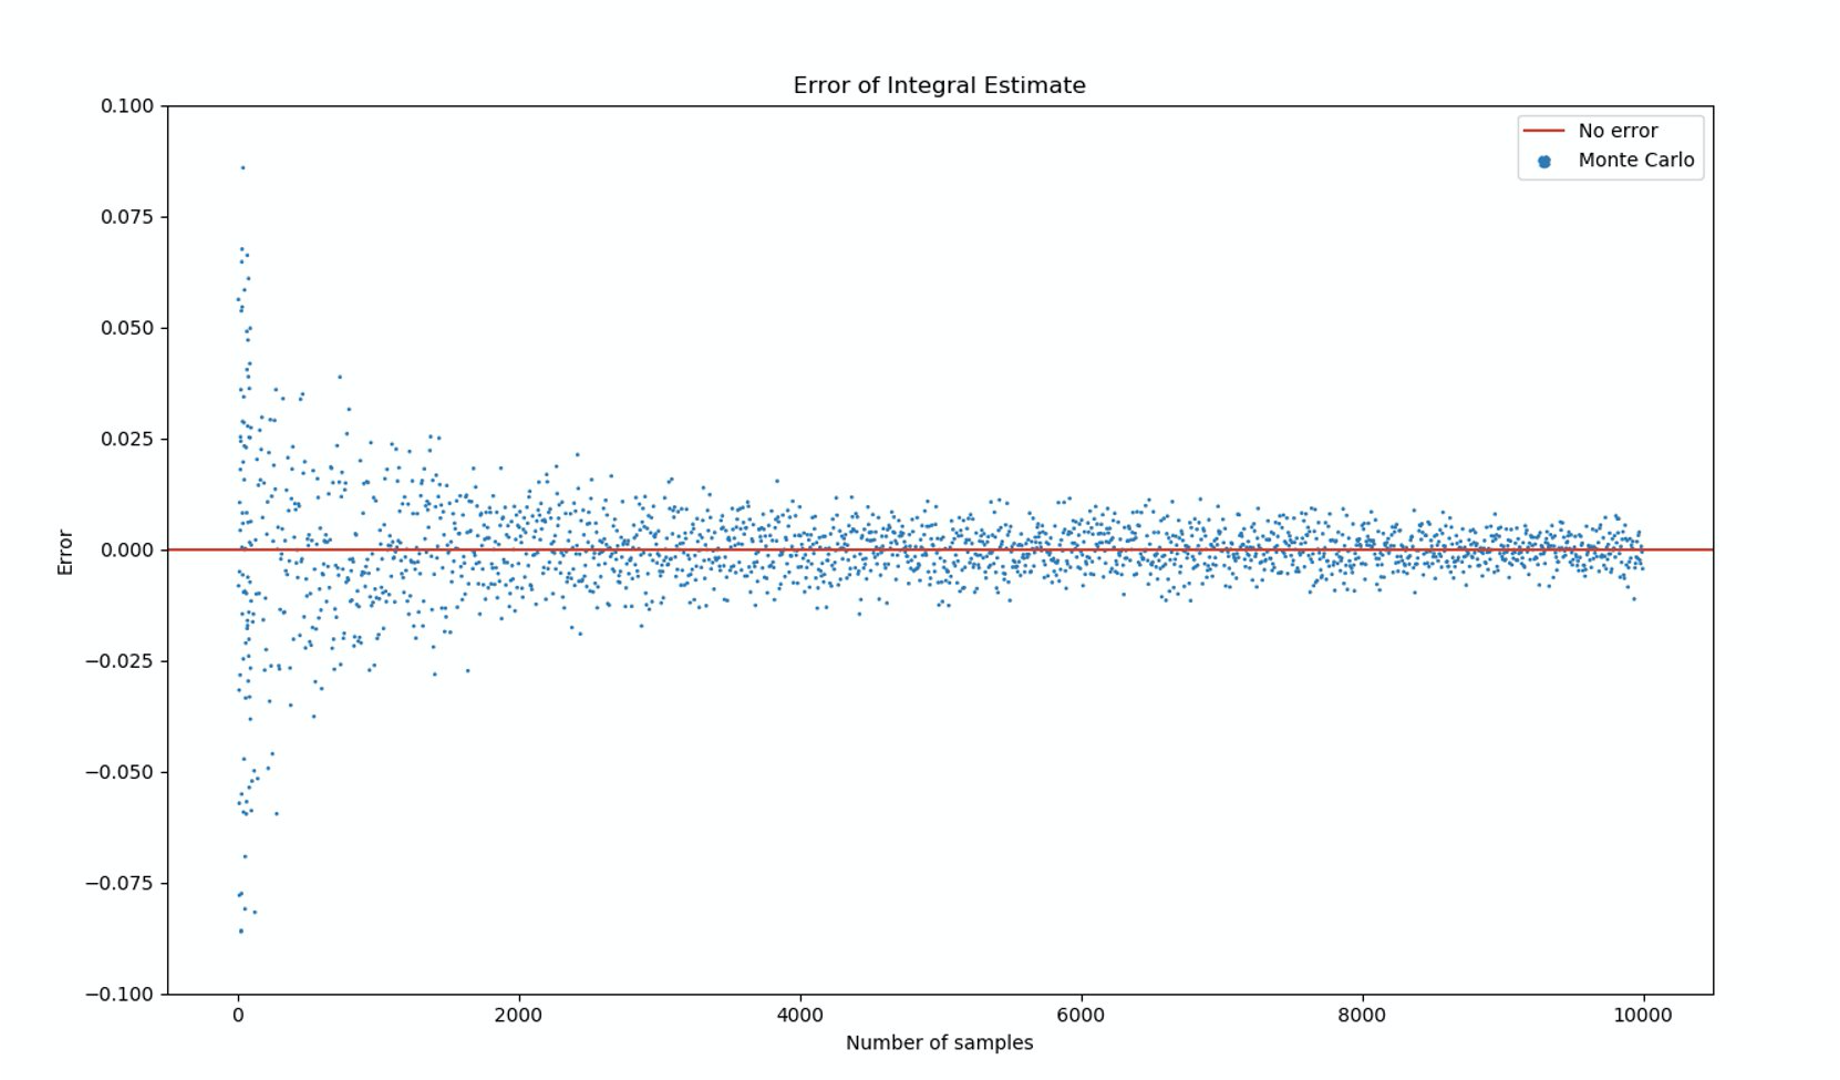
\includegraphics[scale=0.38, center]{Integral_Errors.png}
  \caption{Error of Integral Estimate}
  \label{fig:mc_randomness}
\end{figure}

Although we see a convergence towards a 0 percent error, we still observe estimated values that lie within 0.025 of an error. 

We can extend the Monte Carlo error by comparing it against the Trapezium and Simpsons rule. 

\begin{figure}[h!]
  \includegraphics[scale=0.38, center]{Trap Simp Error.png}
  \caption{Error of Integral Estimate: Simpson's vs Trapezium}
  \label{fig:mc_randomness}
\end{figure}

To observe a difference between all three methods, we can plot on a loglog graph and observe any noticeable difference. 

\begin{figure}[h!]
  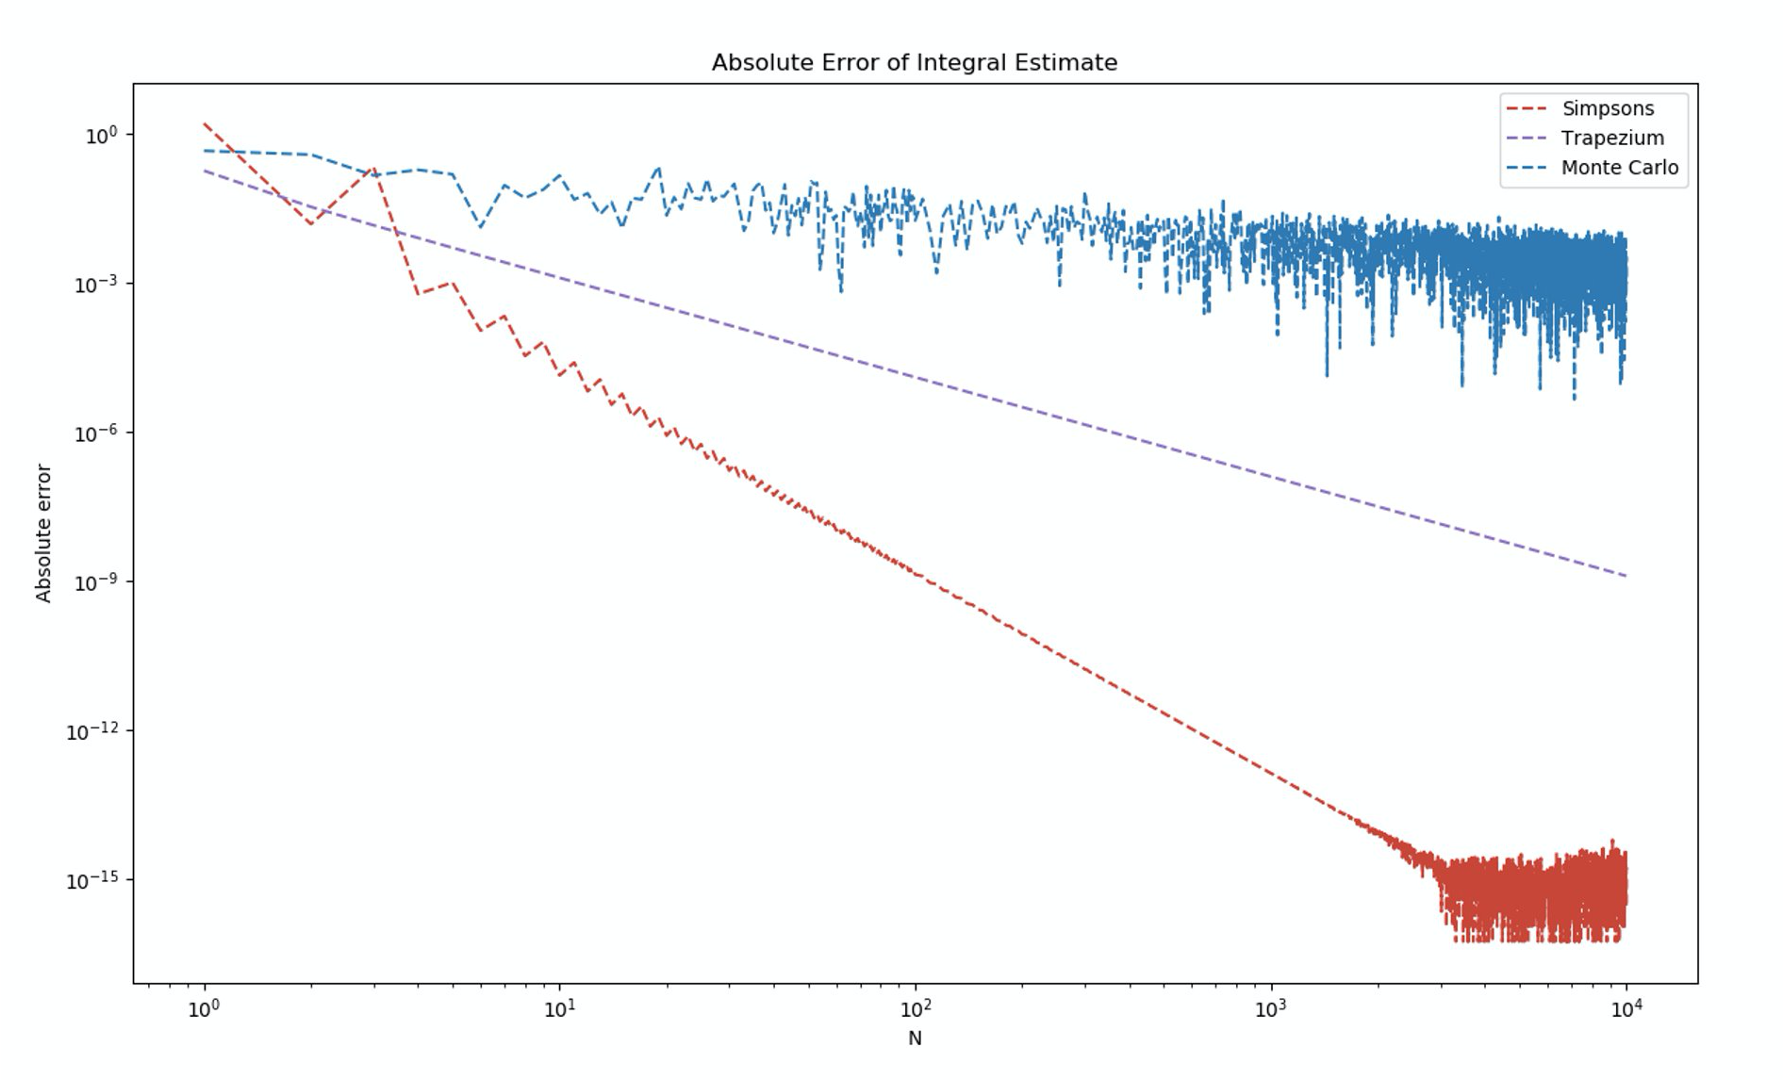
\includegraphics[scale=0.38, center]{loglog_errors.png}
  \caption{Absolute Error of Integral Estimate}
  \label{fig:mc_randomness}
\end{figure}

In Figure 8, we observe that the Simpson's rule (red) converges to a 0 percent error fast than the Trapezium rule (purple). Both these methods also converge faster than the Monte Carlo estimations (blue). Thus, we conclude that for one dimension integration, Simpson's rule is the best followed by Trapezium and Monte Carlo methods. 

\subsection*{Homework Task 3}

Calculate the area of the unit circle by integrating the function,
\begin{align}
f =
\left\{
	\begin{array}{ll}
		1  & \mbox{if } x\textsubscript{1}^2 + x\textsubscript{2}^2 < 1 \\
		0 & \mbox{otherwise}
	\end{array}
\right.
\end{align}
over the domain, $V$ = \{($x\textsubscript{1}$, $x\textsubscript{2}$) : $|x\textsubscript{1}|$ $< 1$, $|x\textsubscript{2}|$ $< 1$\}. 

The answer is of course $\pi$. Write and execute your own program to estimate the integral using Monte-Carlo sampling. By plotting a graph, examine how the error changes with $N$. Run repeated calculations for particular values of N and compare the variance with the error estimator. How many samples would you need to calculate $\pi$ to $3$, $5$ and $10$ decimal places?

\subsubsection*{Answer}

We begin by writing and executing our python code. The results can be seen in the graphs below. In Figure 9, we observe how the estimated integral converges to the actual integral as N is increased. This is a result we already expect.

\begin{figure}[h]
\begin{subfigure}{0.5\textwidth}
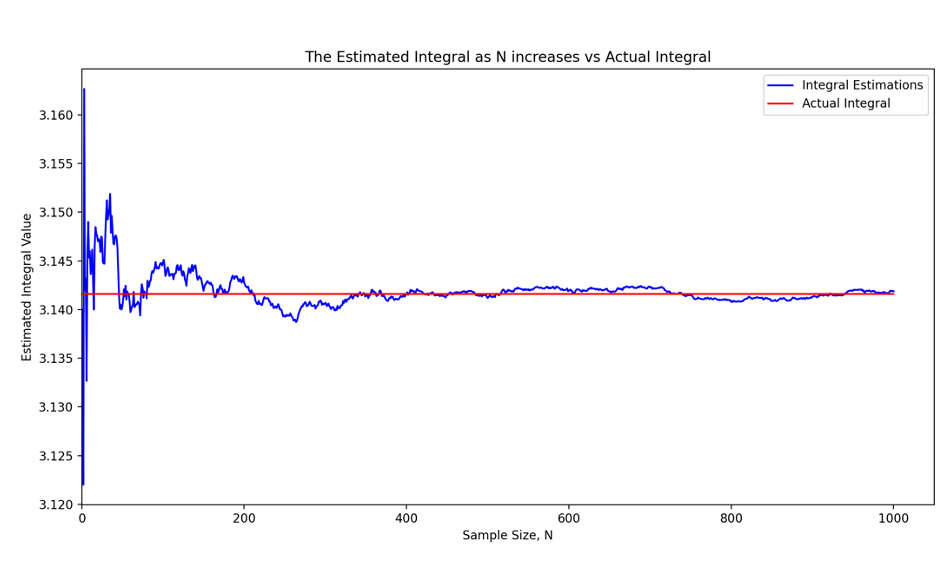
\includegraphics[width=1\linewidth, left]{Integral Estimation vs Actual Integral.png} 
\caption{Without Variance Bounds}
\label{fig:subim1}
\end{subfigure}
\begin{subfigure}{0.5\textwidth}
\includegraphics[width=0.8\linewidth]{unit circle with variance bounds.png}
\caption{With Bounds (Black Bars)}
\label{fig:subim2}
\end{subfigure}
\caption{Estimated Integral vs Actual Integral for Increasing N}
\label{fig:image2}
\end{figure}

We can take the integration estimation further by examining how the error changes with N. In multi-dimensional integration, we know that the error scales as $N^{\frac{-1}{2}}$. Thus, we expect the error to scale in this way. We can observe this by plotting on a normal plot and a loglog plot as can be seen in Figures 10 and 11.

Before we produce plots, we must ensure that we are calculating the error correctly as we are no longer in one dimension. We can use the error given above in Multi-Dimensional Integration to calculate the error for varying $N$ and thus, plot this as seen in Figures 10 and 11. \\


As given in the lecture notes, the error, $E\textsubscript{$N$}$ is defined as;
 \begin{align} 
E\textsubscript{N} = V\frac{\sigma}{\sqrt{N}}
\end{align}
As before, 
\begin{equation}
\sigma =  \sqrt{{\langle f^2\rangle} - {\langle f\rangle ^2}}
\end{equation}

Now, we are working in $V$ = \{($x\textsubscript{1}$, $x\textsubscript{2}$) : $|x\textsubscript{1}|$ $< 1$, $|x\textsubscript{2}|$ $< 1$\}. Thus, $V$ = $4$.\\
Altogether, we obtain;
 \begin{align} 
E\textsubscript{N} = 4 \frac{\sqrt{{\langle f^2\rangle} - {\langle f\rangle ^2}}}{\sqrt{N}}
\end{align}
which we can calculate in python for varying $N$ values. The result of this calculation can be seen in Figure 10 below.

\begin{figure}[h!]
  \includegraphics[scale=0.3, center]{Normal Plot Error Changes with N copy.png}
  \caption{How the Error Changes with N}
  \label{fig:mc_randomness}
\end{figure}

We can now compare this with $N^{\frac{-1}{2}}$ and observe whether our error scales in this way. If it didn't then we know we have done something wrong in our calculations or code!

\begin{figure}[h]
\begin{subfigure}{0.5\textwidth}
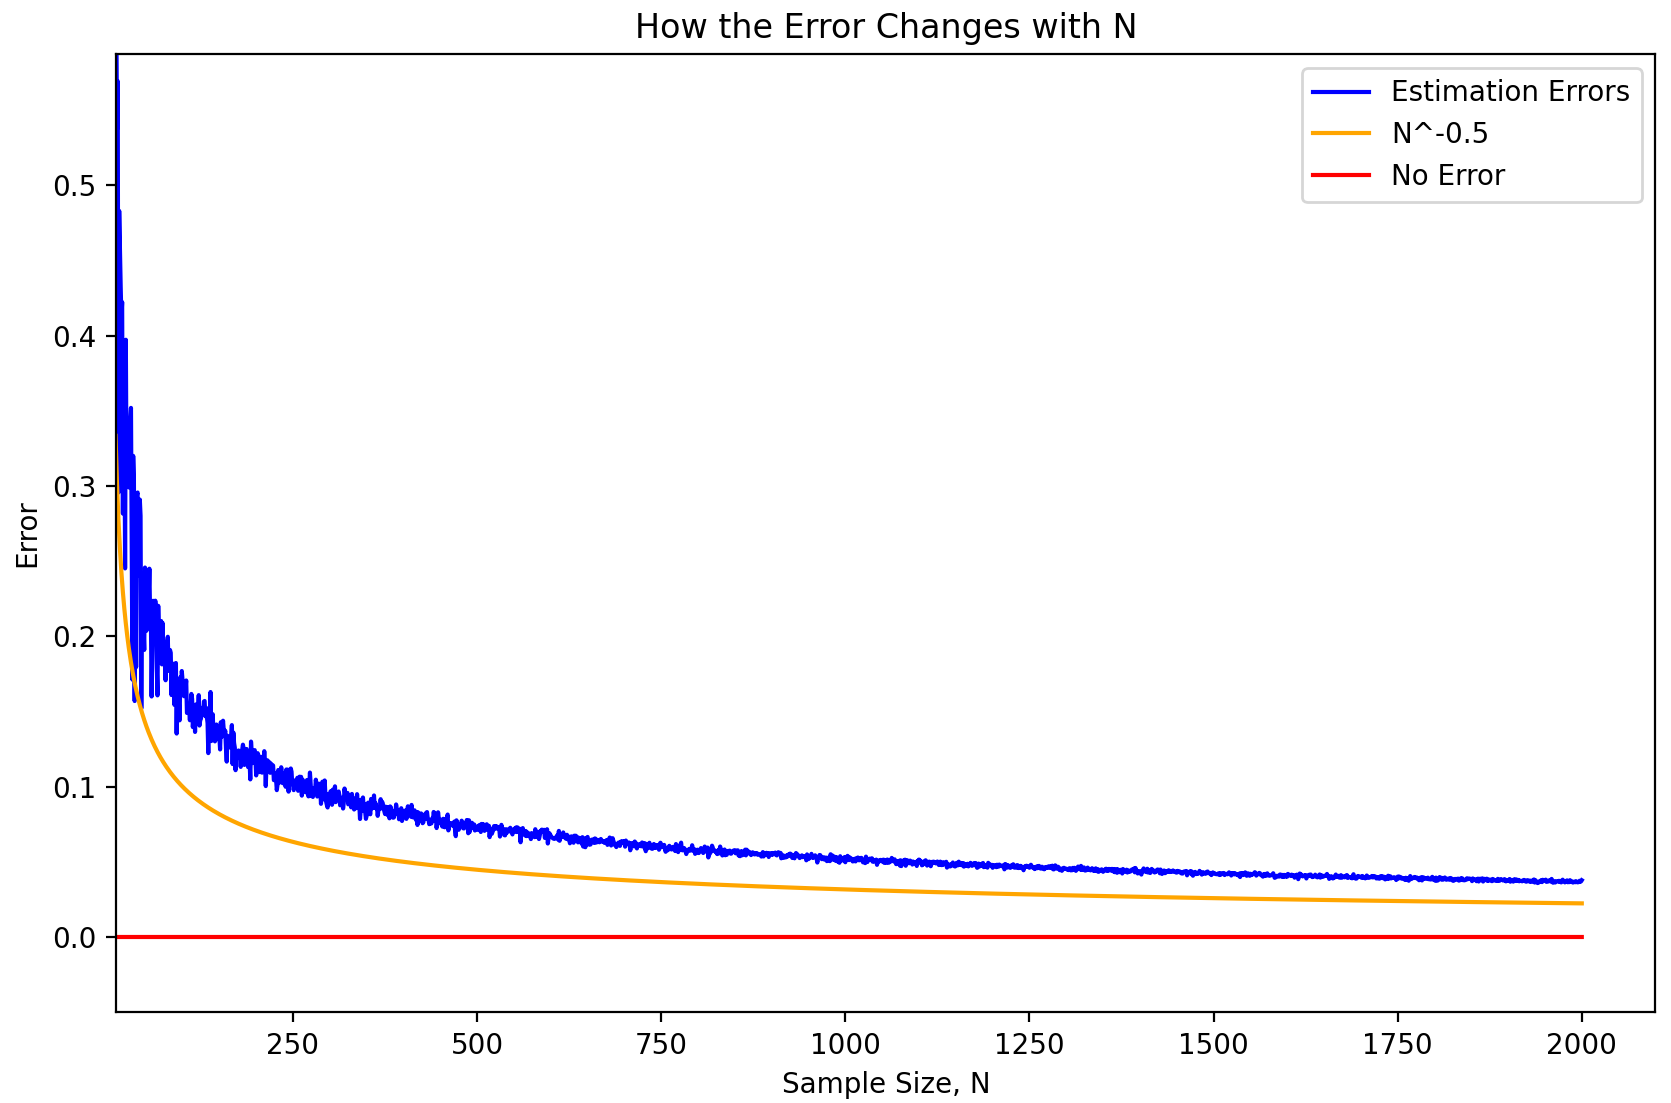
\includegraphics[width=1\linewidth, left]{error vs N normal graph copy.png} 
\caption{Normal Plot}
\label{fig:subim1}
\end{subfigure}
\begin{subfigure}{0.5\textwidth}
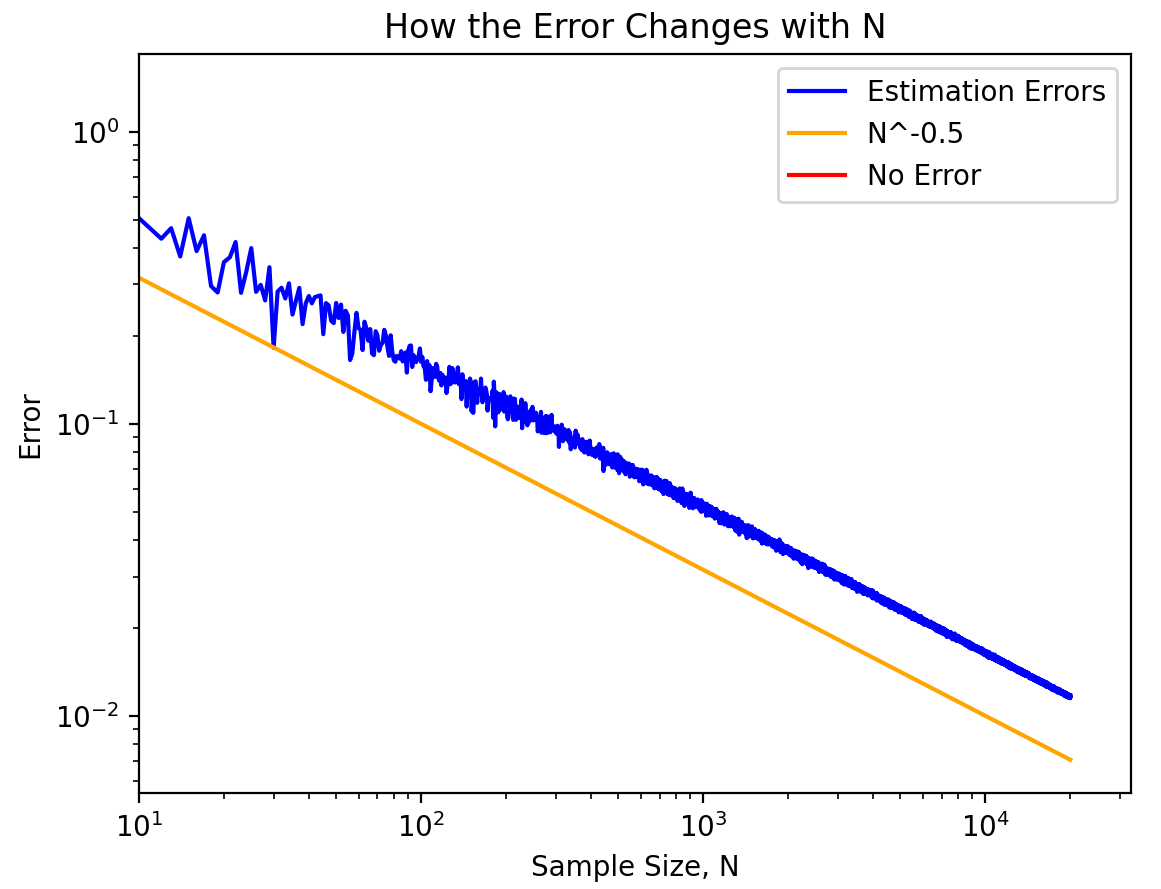
\includegraphics[width=0.9\linewidth]{20,000 copy.png}
\caption{Loglog Plot}
\label{fig:subim2}
\end{subfigure}
\caption{Error vs $N^{\frac{-1}{2}}$}
\label{fig:image2}
\end{figure}

As can be seen in Figure 11, the error scales in the expected way. For increased certainty, we can plot on a loglog graph and observe the behaviour of our estimation error (blue) and $N^{\frac{-1}{2}}$ (orange). 

We can take a more analytic approach and calculate the true variance and the corresponding error. We can then compare this against the error estimation.

By definition,
 \begin{align} 
\sigma^2 = \frac{1}{V}\int f^2 dv \; – \; (\frac{1}{V}\int f dv)^2 = \frac{\pi}{4} \; – \; (\frac{\pi}{4})^2 =  0.1685...
\end{align}

Using the formula for the error, we can calculate the error from the analytic result and observe how this compares with our estimated error. We can also plot the estimated variance against the true varaince.

\begin{figure}[h]
\begin{subfigure}{0.5\textwidth}
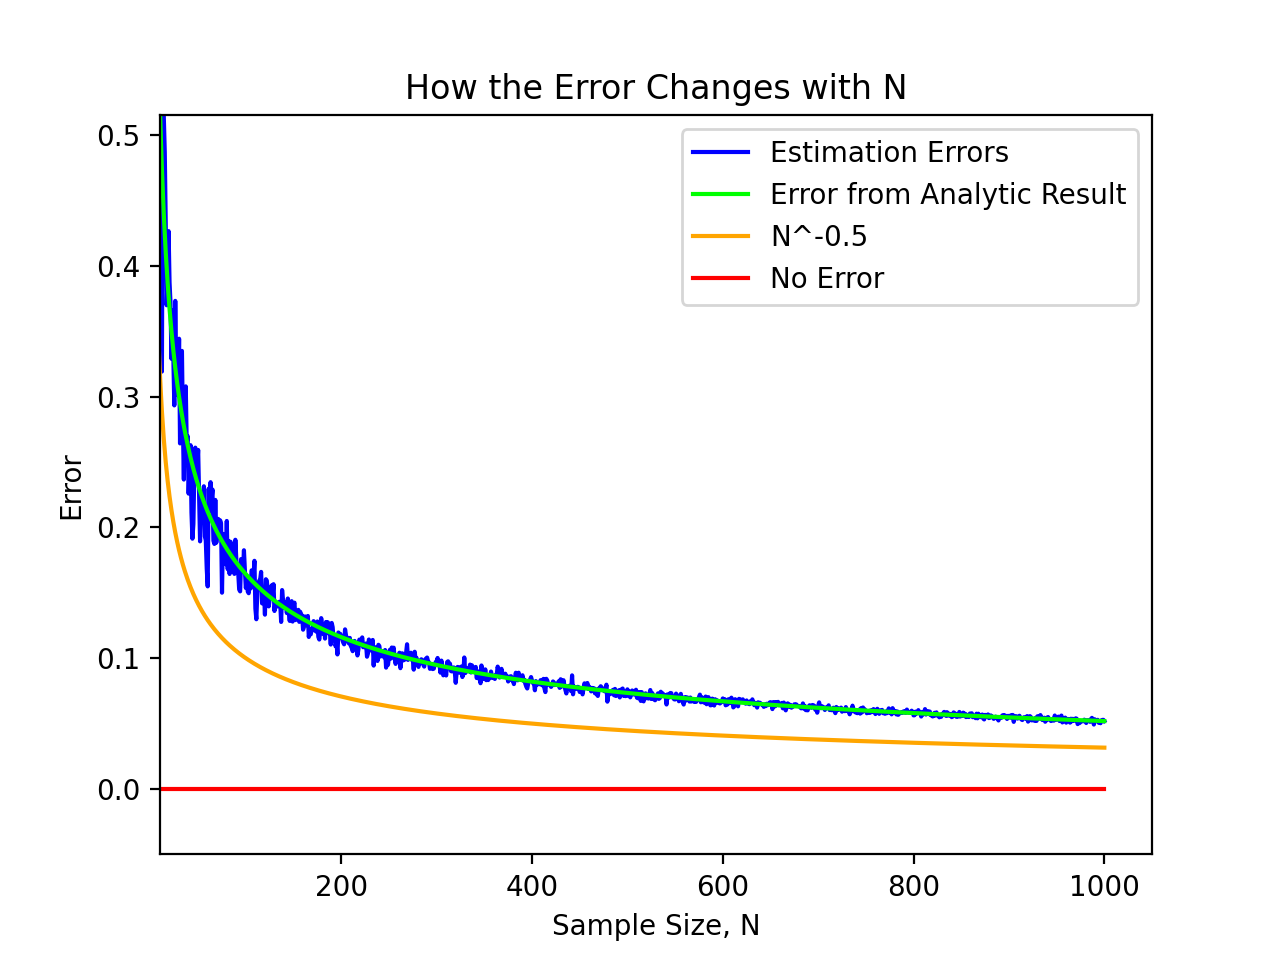
\includegraphics[width=1\linewidth, left]{error from analytic result.png} 
\caption{Error from Analytic Result}
\label{fig:subim1}
\end{subfigure}
\begin{subfigure}{0.5\textwidth}
\includegraphics[width=1\linewidth]{variance.png}
\caption{Estimated Variance}
\label{fig:subim2}
\end{subfigure}
\caption{Comparing Against Analytic Results (True Variance)}
\label{fig:image2}
\end{figure}

We see that the error from an analytic result compares to that of our estimated errors which is a phenomena that we would expect. We also observe that the estimated variance converges to the true variance as expected. 

We can create some order from this randomness and accurately calculate the value of $N$ for a given error. 

So, define
 \begin{align} 
F\textsubscript{N} = \frac{1}{N}\sum_{i=1}^{N} f(x_{i})\,
\end{align}

By the Central Limit Theorem, we can derive,
 \begin{align} 
F\textsubscript{N} \overset{d}{\longrightarrow}  \mathcal{N}(\;\langle f\rangle,\;\frac{\sigma}{\sqrt{N}}\;)
\end{align}
as $N$ tends towards infinity. The proof is identical to the one dimensional case but we replace $(b - a)$ with $V$. In our example, $V = 4$.

Hence, for large $N$ there is (approximately) a 95\% probability that $F\textsubscript{N}$ lies within 2 standard deviations of the mean value of f, $\langle f\rangle$. That is, 
 \begin{align} 
F\textsubscript{N} \in \Big[\langle f\rangle - \frac{\sigma}{\sqrt{N}} , \langle f\rangle + \frac{\sigma}{\sqrt{N}} \Big]
\end{align}

We have seen above that the true variance is 0.1685 to 4 decimal places. Hence, we can get a 95\% confidence interval for $F\textsubscript{N} $ which is our estimate for  $\langle f\rangle$.

We can use this to approximate N such that there's a 95\% probability that our Monte Carlo integration estimate lies within a desired distance of the true value of the integral.

We choose N such that,
 \begin{align} 
\frac{2\sigma}{\sqrt{N}} \leq \frac{y}{V} \implies N \geq \frac{4 V ^2\sigma}{y^2}
\end{align}

In Python, we take the smallest such N that satisfies:
 \begin{align} 
N = \Bigg[ \frac{4 V ^2\sigma}{y^2} \Bigg]
\end{align}

For this value of N, there is a 95\% probability that,
 \begin{align} 
F\textsubscript{N} \in \Big[\langle f\rangle - \frac{y}{\sqrt{N}} , \langle f\rangle + \frac{y}{\sqrt{N}} \Big]\\
\\
\implies V \cdot F\textsubscript{N} \in [V\langle f\rangle - y, V \langle f\rangle + y]
\end{align}

Hence, our Monte Carlo estimate is within distance y (e.g y = 0.01) of the true value of the integral.

Programming this in Python, we calculate N such that there's a 95\% probability that our estimate 
is correct to 3, 5 and 10 decimal places.

Thus, 

3 decimal places: 1,078,706,486 

5 decimal places: 10,787,064,853,080 

10 decimal places: 107,870,648,530,792,590,868,480 

\pagebreak

\subsection*{Chapter 3 - Molecules in Materials}

There is one particular application in which high-dimensional Monte Carlo sampling is very widely
and successfully used: to model the behaviour of atoms and molecules within a material such as a
fluid.

Specific Monte Carlo methods have been developed to deal with the particular problems
encountered in modelling physical materials — one such method is the “Metropolis Monte Carlo”
scheme, which we shall study in detail. You will learn to use and adapt a Metropolis algorithm to
evaluate some properties of simple thermal systems.


\subsection*{3.1 The Boltzmann Distribution}

Many times in physics we deal with a large number of interacting objects, with a large number of degrees of freedom. For example, we might consider a material made up of many atoms. Then the degrees of freedom would be the positions of each of the atoms in the material.

A microstate of the system is a particular configuration defined by a set of values for the degrees of freedom. For example, if the “system” is a single particle moving in one dimension then each microstate is a different position of the particle. If the system is a set of particles, then each microstate is a different arrangement of those particles, represented by the set of vectors giving the particle positions.

A key result from statistical mechanics is that the probability $p\textsubscript{$i$}$ of finding a physical system in a given microstate $i$ is given (subject to some conditions) by the Boltzmann distribution,
 \begin{align} 
p\textsubscript{i} = A\exp \Big( - \frac{E\textsubscript{i}}{k\textsubscript{B} T}\Big)
\end{align}

$E\textsubscript{i}$ is the energy of state $i$ \\
$T$ is the $absolute$ $temperature$ (usually measured in Kelvin T = 273 $T\textsubscript{C}$
where $T\textsubscript{C}$ is the temperature in Celsius) \\
$k\textsubscript{B}$ is the $Boltzmann's constant$ ($k\textsubscript{B} = 1.38 x 10^{-23}JK^{-1}$ in standard units). \\
$k\textsubscript{B}T$ is the thermal energy associated with a degree of freedom

Now, the normalisation condition says that,
 \begin{align} 
\sum_{i}^{} p_{i}\, \equiv 1
\end{align}

Therefore, 
 \begin{align} 
A^{-1} = \sum_{i}^{} \exp \Big( - \frac{E\textsubscript{i}}{k\textsubscript{B} T}\Big)\,
\end{align}

Notice that states with lower energy are more likely than states with high energy. Very high energy
states with $E_{i}$ \(\gg\) $k_{B}T$ are unlikely to an exponentially small degree.

Supposing we wanted to find the average of some quantity $f$ which depended upon the configuration
(i.e. the microstate) of the system.

Read page 7 of the lecture notes to understand why we cannot find the average of the quantity $f$ and instead, we need to use statistical sampling.

\subsection*{3.2 Metropolis Algorithm}

Add in information about the Metropolis Algorithm.

\subsection*{Homework Task 5: Theory}

Can you show why the algorithm works? You need to consider the idea of detailed balance.

\subsubsection*{Answer}

In the original Metropolis paper, it states,

 \begin{quotation}
‘‘Let the a priori probability that the move will carry a system in state $r$ to state $s$ be $P_{r s}$, 
First, it is clear that $P_{r s} = P_{s r}$, since according to the way our game is played
a particle is equally likely to be moved anywhere within a square of side $2a$ centered about its 
original position. Thus, if states $r$ and $s$ differ from each other only by the position of the particle
 moved and if these positions are within each other's squares, the transition probabilities are equal; 
 otherwise they are zero."
 \end{quotation}
 
 A more rigorous consideration of detailed balance:
 
 In Step 5, we decide whether to accept the change of state or remain in the current state. 
 
 If $\triangle{E_{i j}} \leq 0$ then we accept the change of state and this has probability 1.
 
 If $\triangle{E_{i j}} > 0$ we accept the change of state only with the probability, 
 \begin{align} 
q_{i j} = \exp \Big(-\frac{\triangle{E_{i j}}}{k\textsubscript{B} T}\Big)
\end{align}
 
 Thus, the probability of accepting a move is given by,
  \begin{align} 
\alpha_{i j} = \min \bigg\{ 1, \exp \Big(-\frac{\triangle{E_{i j}}}{k\textsubscript{B} T}\Big) \bigg\}
\end{align}

We know, 
 \begin{align} 
p\textsubscript{i} = A\exp \Big( - \frac{E\textsubscript{i}}{k\textsubscript{B} T}\Big)
\end{align}

So,
 \begin{align} 
\exp \Big(-\frac{\triangle{E_{i j}}}{k\textsubscript{B} T}\Big) = 
\frac{\exp \Big( - \frac{E\textsubscript{j}}{k\textsubscript{B} T}\Big)}{
\exp \Big( - \frac{E\textsubscript{i}}{k\textsubscript{B} T}\Big)} = 
\frac{\frac{p_{j}}{A}}{\frac{p_{i}}{A}} =
\frac{p_{j}}{p_{i}}
 \end{align}
 
Thus, the probability of accepting a move is given by, 
\begin{align} 
\alpha_{i j} = \min \bigg\{ 1, \frac{p_{j}}{p_{i}} \bigg\}
\end{align}
and we assume $p_{j} < p_{i}$ for $\alpha_{i j} \not\equiv 1$.

Now, when the system comes to a steady state then the probability that a given loop through the algorithm takes you from state $i$ to state $j$ is,
\begin{align} 
p_{i}q_{i j} = p_{j}q_{ji}
\end{align}
Let's suppose we attempt to move from state $i$ to state $j$ with probability $a_{i j}$ and as before, we accept this move with probability $\alpha_{i j}$. So, 
\begin{align} 
q_{ij} = a_{ij}\alpha_{ij}
\end{align}
Altogether, 
\begin{align} 
p_{i}q_{i j} &= p_{j}q_{ji} \\
\implies p_{i}a_{i j}\alpha_{i j} &= p_{j}a_{j i}\alpha_{j i}
\end{align}
Now, by the definition of $\alpha$, $\alpha_{i j} = \frac{p_{j}}{p_{i}}$ and $\alpha_{j i} = 1$.
\begin{align} 
\implies p_{i}a_{i j} \frac{p_{j}}{p_{i}} &= p_{j}a_{j i} \\
\implies \; \; \; p_{j}a_{i j} &= p_{j}a_{j i} \\
\implies \; \; \; \; \; \; a_{i j} &= a_{j i} \\
\end{align}
Thus, the probability of going from state $i$ to state $j$ is the same as going from state $j$ to state $i$. Thus, detailed balance is conserved. 

\subsection*{Homework Task 6: Simulation}

The code metropolisquad.py is a simple Python code implementing the Metropo- lis algorithm for a particle moving in a quadratic energy well in 1D. It collects data for the frequency with which the particle visits various locations, and outputs data for a histogram of particle positions in a results file. Take a look at the code. See if you can see how it works. Have a play with the code - can you see what the effect of choosing large or small step size is? Set up the code so that it measures the average position of the particle? Measure the variance in particle position? Try a different energy profile - does the code still give the correct probability distribution? Can you break the algorithm - can you come up with a combination of a energy profile and a step size which means that parts of the energy profile are not visited (e.g. what if there is a large energy barrier between two minima)?

\subsubsection*{Answer}

First, we observe the effect of choosing a large or small step size. For appropriate values of the step size, we observe the distribution following the normal distribution as expected.

\begin{figure}[h!]
  \includegraphics[scale=0.4, center]{N = 10,000 Step = 1.png}
  \caption{Metropolis Monte Carlo Sampling (N = 10,000, Step = 1)}
  \label{fig:mc_randomness}
\end{figure}

We can extend this further by comparing the particle positions against the average particle position. 

\begin{figure}[h!]
  \includegraphics[scale=0.4, center]{Particle Positions Step = 1.png}
  \caption{Particle Positions as N Increases (N = 10,000, Step = 1)}
  \label{fig:mc_randomness}
\end{figure}

Despite particle position fluctuation, we see that the particle positions centre around the average particle position.

We now observe large and small step sizes and their effect on the particle position and overall distribution.

We increase the step size to $200$ 

\begin{figure}[h]
\begin{subfigure}{0.5\textwidth}
\includegraphics[width=1.1\linewidth, left]{N = 10,000, Step = 200.png} 
\caption{Distribution vs Expected Distribution}
\label{fig:subim1}
\end{subfigure}
\begin{subfigure}{0.5\textwidth}
\includegraphics[width=1\linewidth]{Particle Positions Step = 200.png}
\caption{Particle Positions as N Increases}
\label{fig:subim2}
\end{subfigure}
\caption{N = 10,000, Step Size = 200}
\label{fig:image2}
\end{figure}

For a step size of 200, we observe the distribution poorly resembling that of the Normal Distribution. However, the particle positions fluctuate above and below but generally centre around the average particle position. This corresponds with the Normal Distribution mean which can be seen by the large bin width around the centre. 

Similarly, we can observe the effect of choosing a small value of the step size. This time, choosing 0.01.

\begin{figure}[h]
\begin{subfigure}{0.5\textwidth}
\includegraphics[width=1\linewidth, left]{N = 10,000 Step 1 over 100.png} 
\caption{Distribution vs Expected Distribution}
\label{fig:subim1}
\end{subfigure}
\begin{subfigure}{0.5\textwidth}
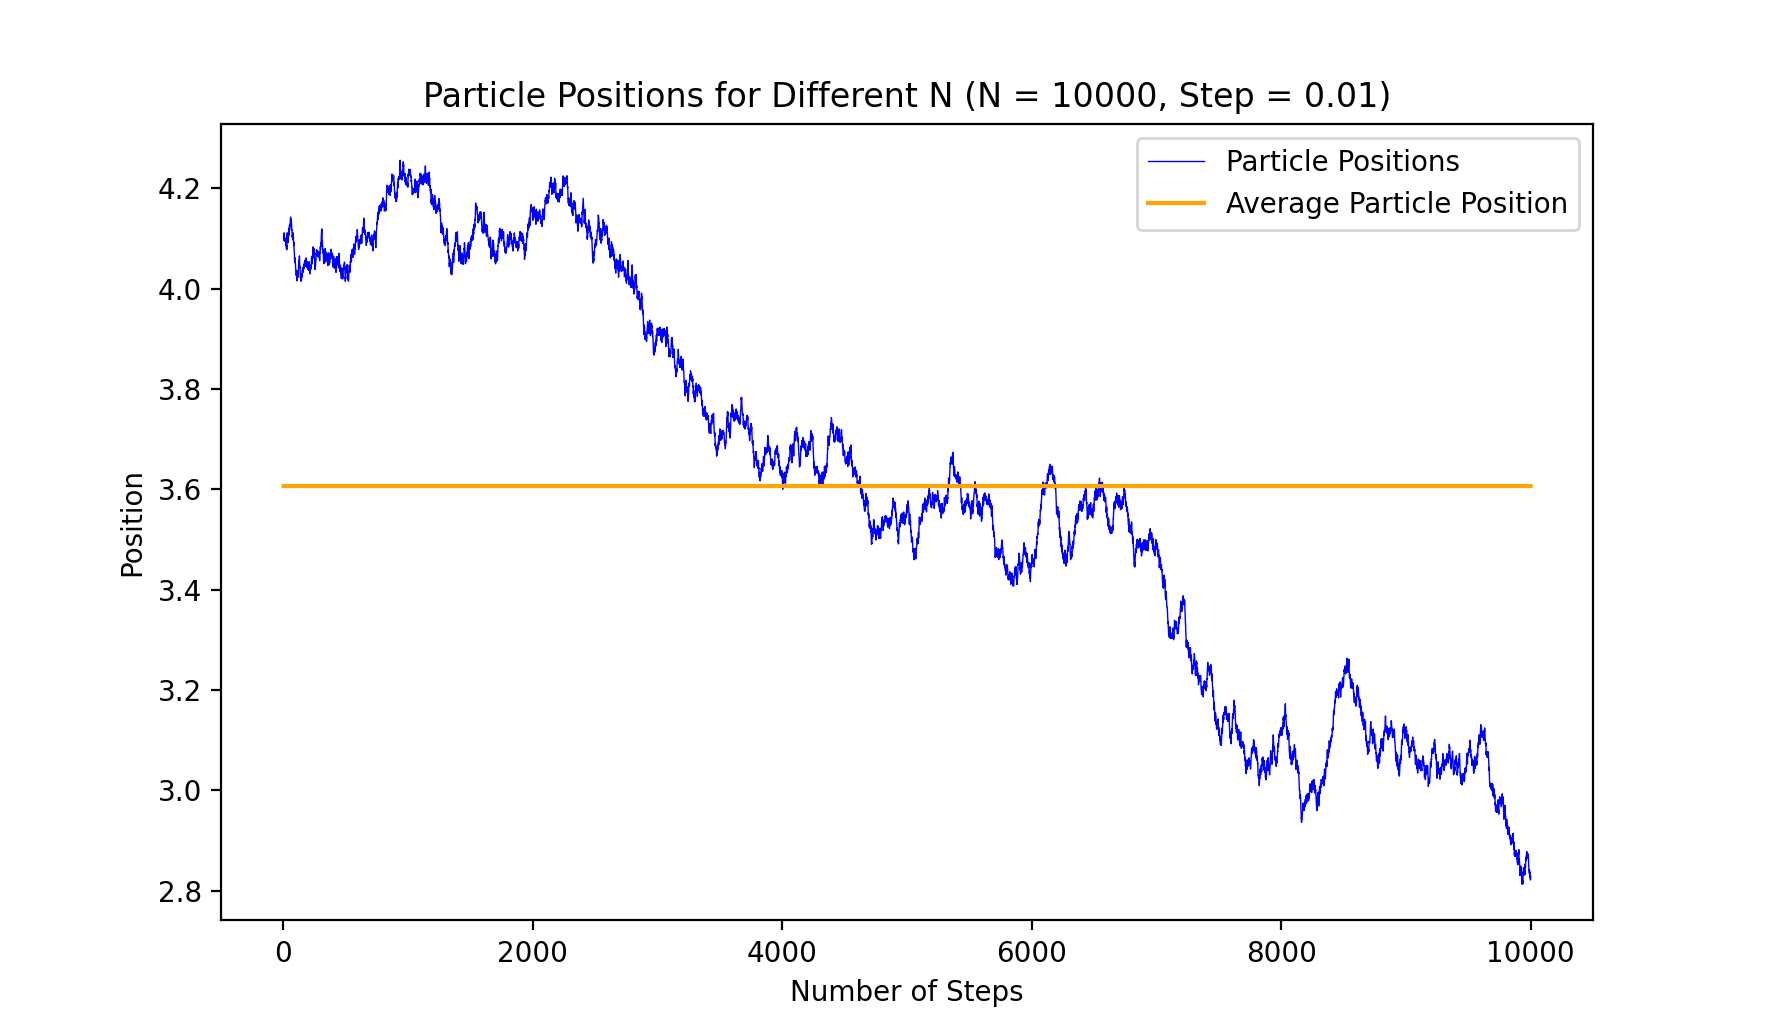
\includegraphics[width=1.05\linewidth]{1 over 100 particle position.png}
\caption{Particle Positions as N Increases}
\label{fig:subim2}
\end{subfigure}
\caption{N = 10,000, Step Size = 0.01}
\label{fig:image2}
\end{figure}

We observe that choosing a significantly small step size reduces the likelihood that the distribution will follow that of a Normal Distribution. 

We can adapt the code to measure the average position of the particle and variance.

Over time the probability of finding the system in a given state after step 5 of the Metropolis Algorithm (irrespective of whether the last random change was accepted or not) should be given by the Boltzmann probability distribution. This means that, for example, to estimate the average of some quantity $f$ we can simply evaluate:
 \begin{align} 
\langle f \rangle = \frac{1}{N}\sum_{i}^{} f_{i}\,
\end{align}
and thus, we can calculate the variance in the way we have done previously. 

As an example of calculating the average position of the particle, Figure 17 demonstrates the average position of the particle as N increases. We can simulate something similar for the variance.

\begin{figure}[h!]
  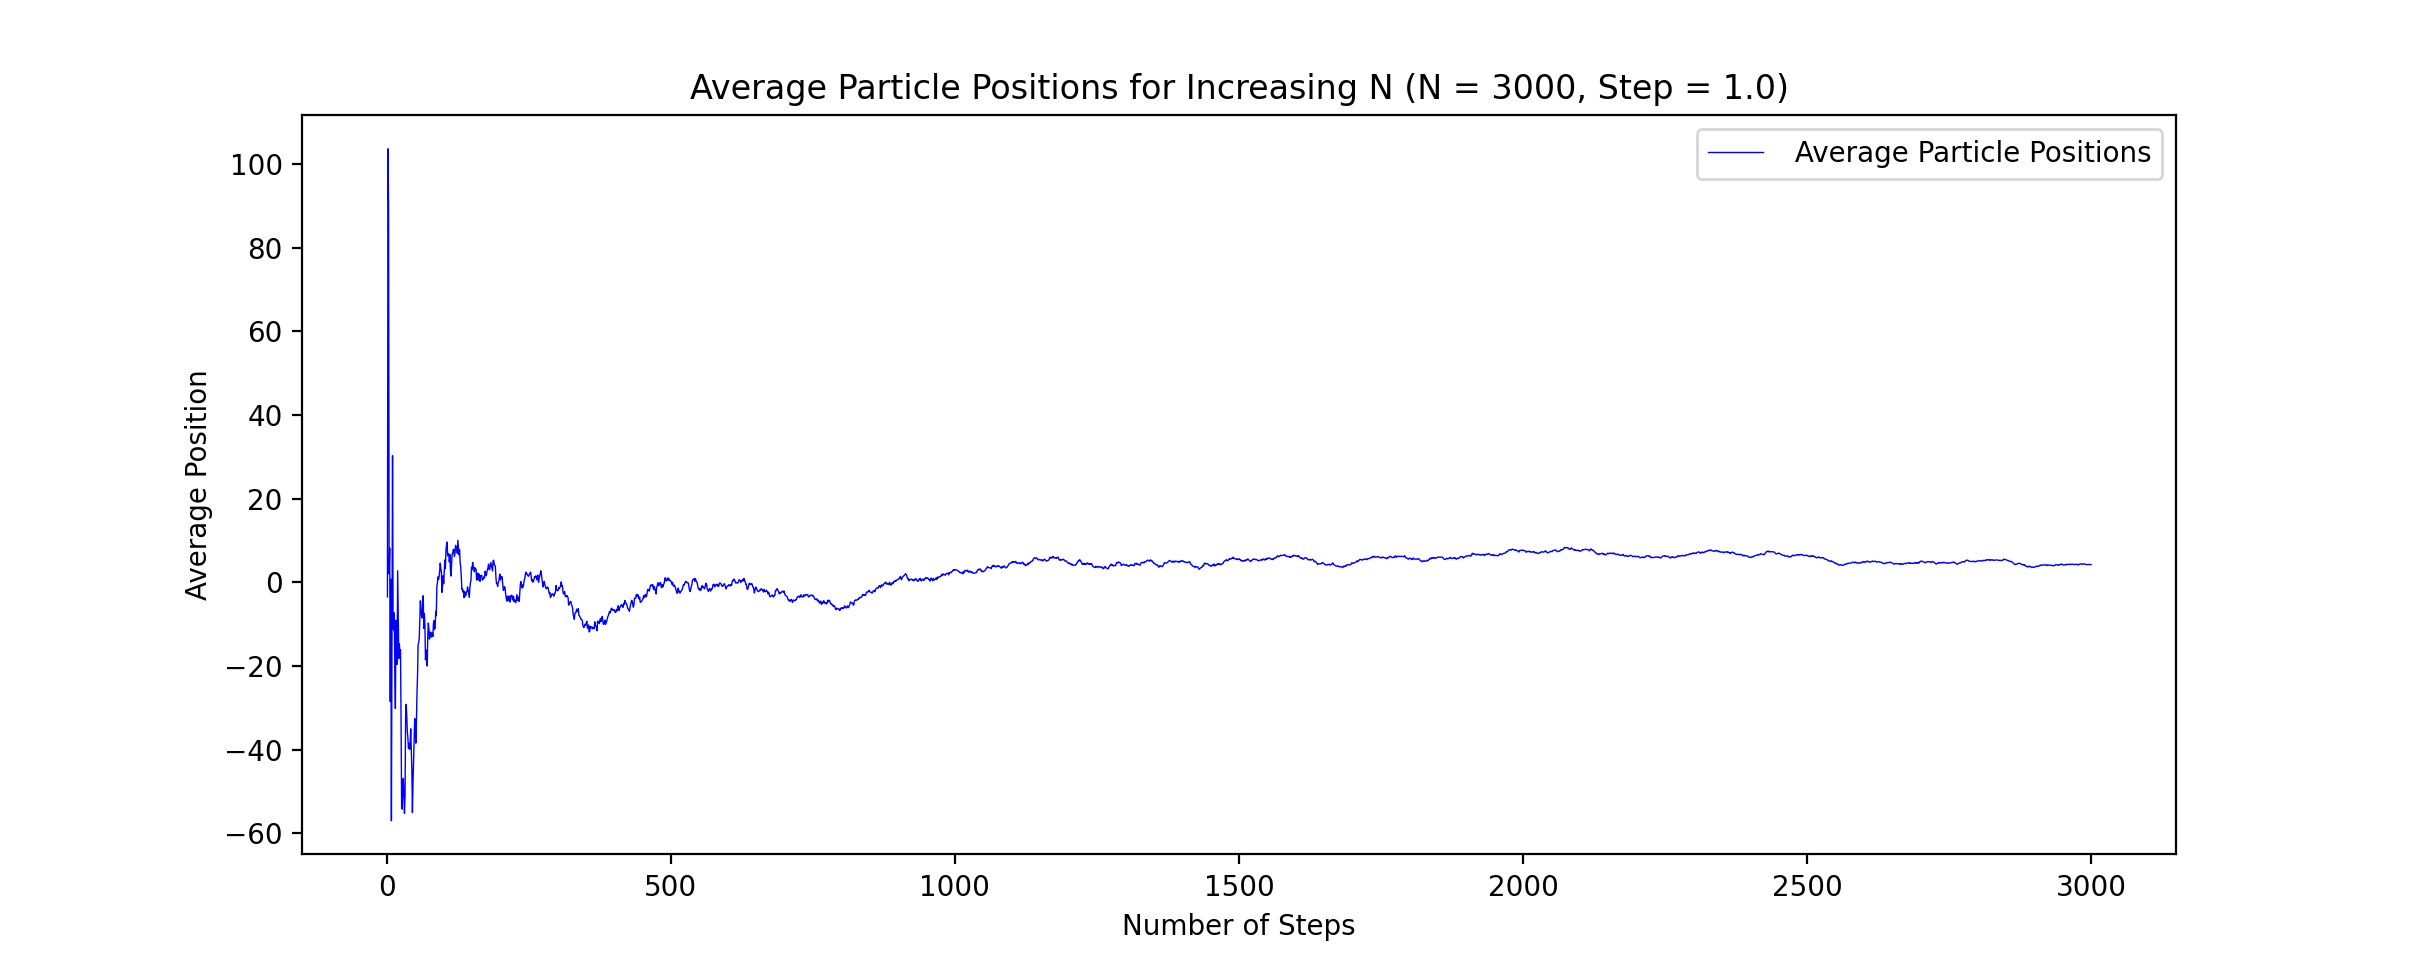
\includegraphics[scale=0.45, center]{average particle position for increasing N.png}
  \caption{Average Particle Positions as N Increases}
  \label{fig:mc_randomness}
\end{figure}

Changing the energy profile results in a change of expected distribution. If you increase the spring constant to a large value, there are subsequently less bins and so the distribution is taller and thinner. Conversely, if you use a decimal (say 0.01) for the spring constant, the number of bins increases and the expected distribution because wider and smaller.

Is it possible to break the algorithm?

Let's first consider the algorithm. So, we define the energy as,
 \begin{align} 
E = \frac{kx^2}{2}
\end{align}
where $k$ is the spring constant and $x$ is the position of the particle.

We begin with $x_{old} = 4.1$, so we can define our old energy as the following,
 \begin{align} 
E_{old} = \frac{4.1^2 k}{2}
\end{align}
Now, the new particle position, $x_{new}$, is defined in the python algorithm as the following,
 \begin{align} 
x_{new} = x_{old} + (Sr)
\end{align}
where $S$ is the number of steps and $r$ is a random number obtained from $\sim U(-1,1)\,$.
So,
 \begin{align} 
E_{new} = \frac{(x_{old} + Sr)^2k}{2}
\end{align}
Then, altogether, we obtain,
 \begin{align} 
E_{diff} = \frac{(4.1 + Sr)^2k}{2} - \frac{4.1^2 k}{2}
\end{align}
For the algorithm to break, we could stay in the same position forever. So, we consider this case.

First, let's assume the steps tend towards 0. In other words, $S \to \infty$. Thus, 
 \begin{align} 
E_{diff} = \triangle{E} \to \infty
\end{align}

Thus, the probability of accepting a move between states is given by, 
\begin{align} 
\alpha = \min \bigg\{ 1, \exp \Big(-\frac{\triangle{E}}{k\textsubscript{B} T}\Big) \bigg\}
\end{align}
Given, $\triangle{E_{i j}} \to \infty$, this reduces to, 
\begin{align} 
\alpha &= \min \{ 1, 0\} \\
\implies \alpha &= 0
\end{align}
So, the probability of accepting a move between states is 0. This means the state remains in the given position forever. 

We can simulate this in Python. We choose our spring constant as $10,000,000$ and our step size as $0.00001$. This can be seen in Figure 18.

\begin{figure}[h!]
  \includegraphics[scale=0.5, center]{remains in the same position.png}
  \caption{Average Particle Positions as N Increases}
  \label{fig:mc_randomness}
\end{figure}

\end{document}

















